\documentclass[sigconf]{acmart} 

% --- Encoding and Fonts ---
\usepackage[utf8]{inputenc} 
\usepackage[T1]{fontenc} 
\usepackage{lmodern} 

% --- Table Packages ---
\usepackage{tabularx} 
\usepackage{array} 
\usepackage{caption} 

% --- Optional but recommended for academic papers ---
\usepackage{hyperref} 
\usepackage{booktabs} 
\usepackage{float}
\usepackage{enumitem}

\usepackage{subcaption}
\usepackage{caption}
\usepackage{xparse}
\usepackage{graphicx}

\usepackage{pgfplots}
\pgfplotsset{compat=1.18}

\renewcommand{\topfraction}{0.9}
\renewcommand{\bottomfraction}{0.8}
\renewcommand{\textfraction}{0.1}
\renewcommand{\floatpagefraction}{0.8}
% Reduce space above and below floats
\setlength{\floatsep}{8pt plus 2pt minus 2pt}
\setlength{\textfloatsep}{10pt plus 2pt minus 4pt}
\setlength{\intextsep}{8pt plus 2pt minus 2pt}

\begin{document}

\newcommand{\displayimages}[9]{
    \begin{figure}[H]
        \centering

        \begin{subfigure}{0.45\columnwidth}
            \includegraphics[width=\linewidth]{../generated-videos/API/frames/#1_0000#5_/#1_0000#5__02.jpg}
            \caption{#6}
        \end{subfigure}
        ~
        \begin{subfigure}{0.45\columnwidth}
            \includegraphics[width=\linewidth]{../generated-videos/API/frames/#2_0000#5_/#2_0000#5__02.jpg}
            \caption{#7}
        \end{subfigure}

        \vfill

        \begin{subfigure}{0.45\columnwidth}
            \includegraphics[width=\linewidth]{../generated-videos/API/frames/#3_0000#5_/#3_0000#5__02.jpg}
            \caption{#8}
        \end{subfigure}
        ~
        \begin{subfigure}{0.45\columnwidth}
            \includegraphics[width=\linewidth]{../generated-videos/API/frames/#4_0000#5_/#4_0000#5__02.jpg}
            \caption{#9}
        \end{subfigure}
    \end{figure}
}

\newcommand{\displaycontinuousimages}[2]{
    \begin{figure}[H]
        \centering

        \begin{subfigure}{0.45\columnwidth}
            
\includegraphics[width=\linewidth]{../generated-videos/dataset v2/frames/LTX-2_0000#1_/frame_01.jpg}
        \end{subfigure}
        ~
        \begin{subfigure}{0.45\columnwidth}
            
\includegraphics[width=\linewidth]{../generated-videos/dataset v2/frames/LTX-2_0000#1_/frame_03.jpg}
        \end{subfigure}

        \vfill

        \begin{subfigure}{0.45\columnwidth}
            
\includegraphics[width=\linewidth]{../generated-videos/dataset v2/frames/LTX-2_0000#1_/frame_05.jpg}
        \end{subfigure}
        ~
        \begin{subfigure}{0.45\columnwidth}
            
\includegraphics[width=\linewidth]{../generated-videos/dataset v2/frames/LTX-2_0000#1_/frame_08.jpg}
        \end{subfigure}

        \caption{#2}

    \end{figure}
}

\newcommand{\displaycontinuousimagesloc}[2]{
    \begin{figure}[H]
        \centering

        \begin{subfigure}{0.45\columnwidth}
            
\includegraphics[width=\linewidth]{../generated-videos/dataset v2/#1/frames/wan22_i2v/frame_01.jpg}
        \end{subfigure}
        ~
        \begin{subfigure}{0.45\columnwidth}
            
\includegraphics[width=\linewidth]{../generated-videos/dataset v2/#1/frames/wan22_i2v/frame_03.jpg}
        \end{subfigure}

        \vfill

        \begin{subfigure}{0.45\columnwidth}
            
\includegraphics[width=\linewidth]{../generated-videos/dataset v2/#1/frames/wan22_i2v/frame_05.jpg}
        \end{subfigure}
        ~
        \begin{subfigure}{0.45\columnwidth}
            
\includegraphics[width=\linewidth]{../generated-videos/dataset v2/#1/frames/wan22_i2v/frame_08.jpg}
        \end{subfigure}

        \caption{#2}

    \end{figure}
}

\newcommand{\displaycontinuousimagesold}[8]{
    \begin{figure}[h]
        \centering

        \begin{subfigure}{0.45\columnwidth}
            \includegraphics[width=\linewidth]{../generated-videos/#1/frames/#2_0000#3_/#2_0000#3__0#4.jpg}
        \end{subfigure}
        ~
        \begin{subfigure}{0.45\columnwidth}
            \includegraphics[width=\linewidth]{../generated-videos/#1/frames/#2_0000#3_/#2_0000#3__0#5.jpg}
        \end{subfigure}

        \vfill

        \begin{subfigure}{0.45\columnwidth}
            \includegraphics[width=\linewidth]{../generated-videos/#1/frames/#2_0000#3_/#2_0000#3__0#6.jpg}
        \end{subfigure}
        ~
        \begin{subfigure}{0.45\columnwidth}
            \includegraphics[width=\linewidth]{../generated-videos/#1/frames/#2_0000#3_/#2_0000#3__0#7.jpg}
        \end{subfigure}

        \caption{#8}
    \end{figure}
}


\newcommand{\displaylocalimages}[2]{
    \begin{figure}[H]
        \centering

        % Top row — LTX
        \begin{subfigure}{0.45\columnwidth}
            \includegraphics[width=\linewidth]{../generated-videos/local/frames/LTX_2.3_t2v_0000#2_/LTX_2.3_t2v_0000#2__01.jpg}
        \end{subfigure}
        ~
        \begin{subfigure}{0.45\columnwidth}
            \includegraphics[width=\linewidth]{../generated-videos/local/frames/LTX_2.3_t2v_0000#2_/LTX_2.3_t2v_0000#2__04.jpg}
        \end{subfigure}

        \vspace{0.5em}

        \caption*{LTX 2.3}

        \vspace{1em}

        % Bottom row — Wan
        \begin{subfigure}{0.45\columnwidth}
            \includegraphics[width=\linewidth]{../generated-videos/local/frames/ComfyUI_000#1_/ComfyUI_000#1__01.jpg}
        \end{subfigure}
        ~
        \begin{subfigure}{0.45\columnwidth}
            \includegraphics[width=\linewidth]{../generated-videos/local/frames/ComfyUI_000#1_/ComfyUI_000#1__04.jpg}
        \end{subfigure}

        \vspace{0.5em}

        \caption*{Wan 2.2 (14B)}

    \end{figure}
}

\pgfplotsset{custom axis/.style={
            ybar=0pt, % Removes gap between bars in the same group
            bar width=7pt,
            width=\columnwidth,
            height=0.3\textheight, % Increased height for better legibility
            symbolic x coords={Veo, Kling, LTX, Vidu, Seedance, Grok},
            xtick=data,
            ymin=0, ymax=5.5,
            ylabel={Score},
            xlabel={Model},
            % title={Evaluation Scores for Prompt [1] (Red Cube)},
            % Grid and Axis Style
            ymajorgrids=true,
            grid style={dashed, gray!30},
            axis line style={gray!60},
            % Legend Style
            legend style={
                    at={(0.5,-0.2)},
                    anchor=north,
                    legend columns=2,
                    draw=none, % Remove border
                    /tikz/every even column/.append style={column sep=10pt}
                },
            % Label Styles
            nodes near coords,
            every node near coord/.append style={font=\tiny, inner sep=2pt},
            label style={font=\small},
            tick label style={font=\small},
            title style={font=\bfseries\small, yshift=2pt},
            enlarge x limits=0.15,
        }
}


\title{A Survey: Video Generative Models}

\author{Taraash Mittal}
\authornote{Both authors contributed equally to this research.}
\email{taraash23552@iiitd.ac.in}

\author{Utkarsh Garg}
\authornotemark[1]
\email{utkarsh23570@iiitd.ac.in}

\author{Anoop Ratn}
\author{Rajiv Ratn Shah}
\affiliation{%
    \institution{Indraprastha Institute of Information Technology}
    \city{Delhi}
    \country{India}
}

\renewcommand{\shortauthors}{Mittal and Garg, et al.}

\definecolor{color1}{RGB}{31, 119, 180}  % Steel Blue
\definecolor{color2}{RGB}{174, 199, 232} % Light Blue
\definecolor{color3}{RGB}{255, 127, 14}  % Safety Orange
\definecolor{color4}{RGB}{255, 187, 120} % Light Orange

\begin{abstract}
    The rapid evolution of generative artificial intelligence has positioned video generation as the current frontier of creative machine learning models. Despite a recent burst of such architectures, there remains a notable absence of large-scale comparative studies analyzing their practical capabilities. This paper addresses this gap by first underpinning the general inner workings of video generative models, followed by a detailed examination of the unique functional mechanics of each model evaluated in this study. To systematically assess these systems, we introduce a curated list of targeted stress-testing prompts designed to rigorously judge the models' temporal coherence, spatial and physical reasoning, prompt inference accuracy, and animation style lineage. Ultimately, we review the current state of both AI generative video models across a variety of use cases, explicitly testing their individual strengths and weaknesses to evaluate their viability in professional workflows. The dataset will be made public to facilitate future research.
\end{abstract}

\begin{teaserfigure}
    \centering
    
\includegraphics[height=15em]{images/image.png} ~ 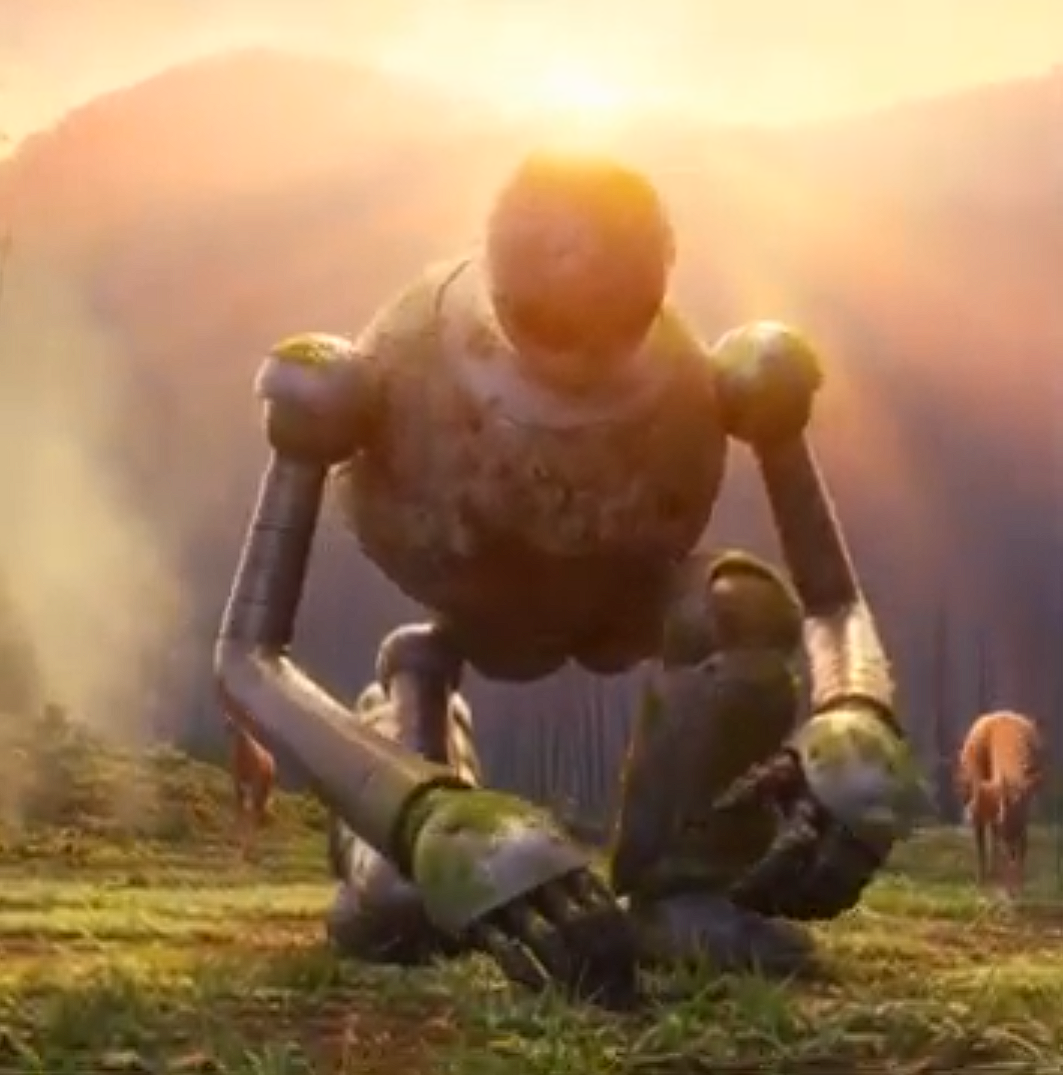
\includegraphics[height=15em]{image.png}
    \caption{Wild Robot (left: real; right: extended using Wan 2.2)}
\end{teaserfigure}

\maketitle
\section{Introduction}
\label{sec:introduction}

The ability to generate video from a text prompt or a single image is no
longer a research curiosity, it is a freely accessible consumer product.
Within seconds, anyone can invoke a state-of-the-art (SOTA) generative
model and receive a video of reasonable visual quality, at little to no
cost. This accessibility has been driven by two parallel forces: the
rapid scaling of proprietary models such as Google's Veo~3 and OpenAI's
Sora \cite{openai2024sora, deepmind2024veo}, which benefit from
substantial computational resources and curated training corpora, and a
thriving open-source ecosystem, represented by models such as Wan~2.2,
Vidu, and LTX, that has narrowed the quality gap despite operating under
significantly tighter resource constraints. The ability to generate complex
temporal media through natural language alone represents a fundamental
shift in creative workflows, with direct implications for rapid
prototyping, previsualization, and cinematographic ideation
\cite{brooks2024sora, yang2024cogvideox}.

Yet visual fidelity alone does not determine whether a model is useful in
a professional pipeline. Integrating generative video into production
workflows demands something more precise: strict adherence to human
instructions, physical plausibility, and consistency of objects,
characters, and lighting across generated frames. A model that produces
a beautiful but physically incoherent shot, or that loses track of a
character's identity mid-sequence, is not a production-viable tool. Despite this, the literature lacks large-scale comparative
studies that evaluate current SOTA models specifically against these
production-relevant criteria \cite{huang2024vbench, liu2024evalcrafter}.
This paper addresses that gap directly.

\begin{figure}[h]
    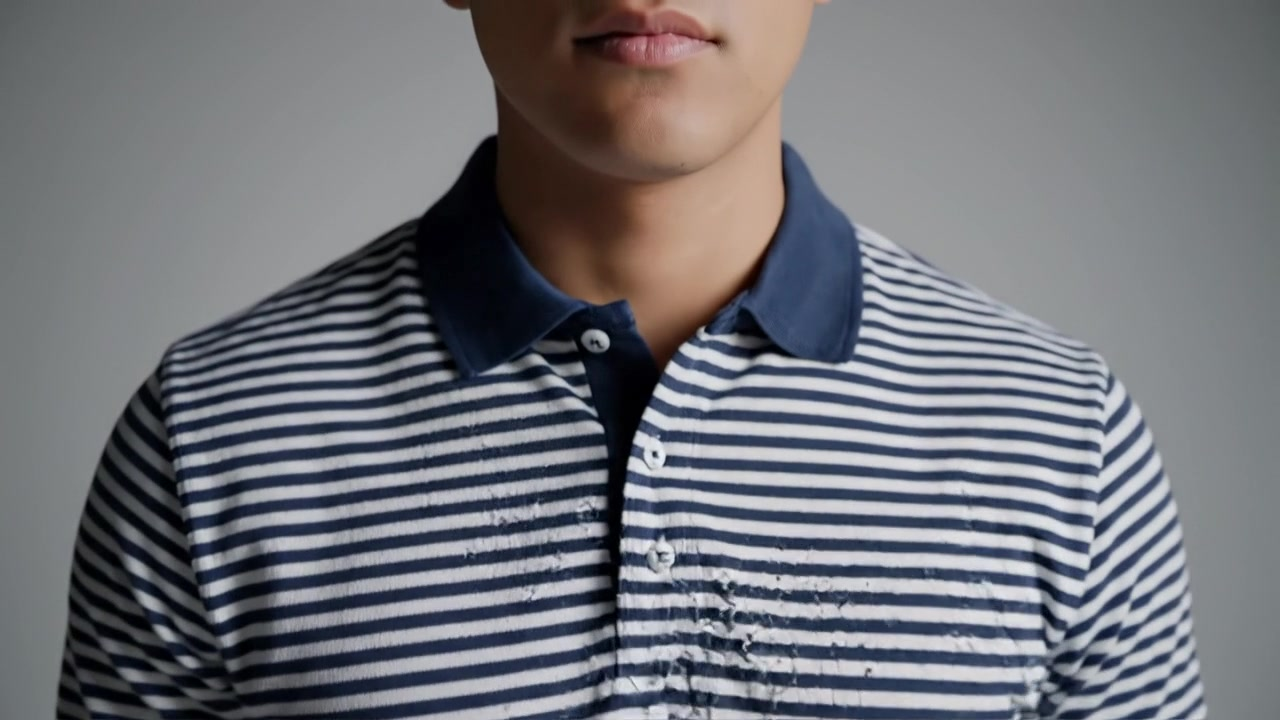
\includegraphics[width=0.7\columnwidth]
    {../generated-videos/API/frames/veo_00004_/veo_00004__03.jpg}
    \caption{Google Veo 3}
\end{figure}

Current SOTA models display impressive visual fidelity, but they face
systematic and reproducible mechanical failures. Models frequently
struggle with object permanence and structural integrity: high-frequency
surface details exhibit 2.5D warping at macro scales rather than
maintaining true 3D geometric persistence, and texture stability breaks
down under even simple camera motion. Temporal consistency remains a
fundamental challenge.

\displaycontinuousimagesold{API}{ltx-t2v}{2}{1}{2}{3}{4}{LTX 2.3}


When tasked with simulating gravity or complex physical interactions,
models can fail catastrophically. A particularly striking failure mode
we document is \textit{object mitosis}: the model entirely loses track
of an object's geometry and mass, causing a single item (such as a
bouncing ball) to erroneously split into two distinct objects
mid-sequence. Even basic Newtonian mechanics, such as elastic rebounds
and kinetic energy decay upon surface contact, expose systematic
weaknesses. In long-horizon coherence tests, rather than rendering
continuous action, models frequently hallucinate new scene states or
resort to severe jump cuts that restart the narrative context entirely.
\begin{figure}[h]
    \centering
    \begin{subfigure}{0.45\columnwidth}
        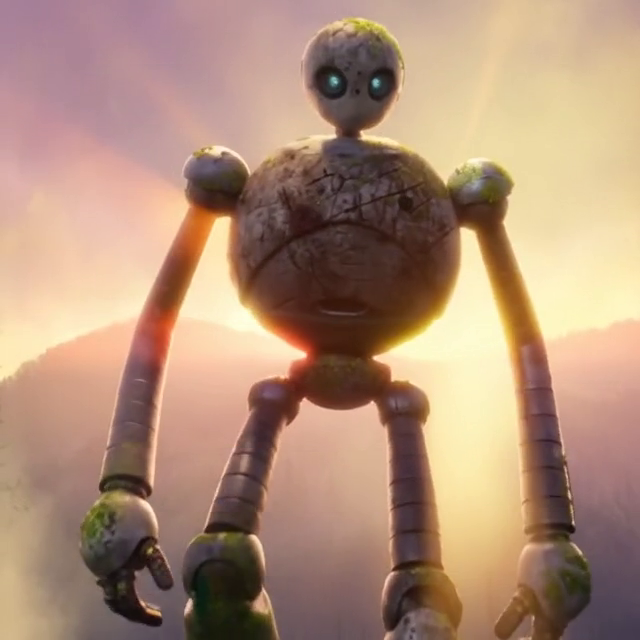
\includegraphics[width=\linewidth]
        {../generated-videos/dataset v2/wil1/wan22_i2v/frame_002.png}
    \end{subfigure}
    ~
    \begin{subfigure}{0.45\columnwidth}
        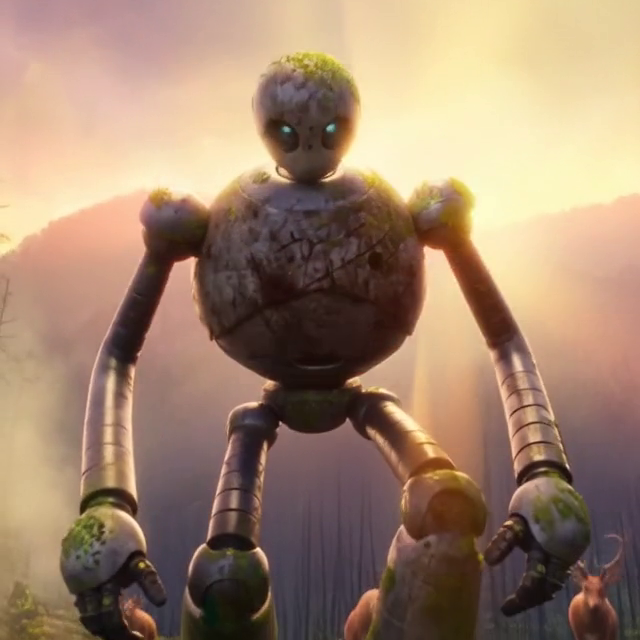
\includegraphics[width=\linewidth]
        {../generated-videos/dataset v2/wil1/wan22_i2v/frame_004.png}
    \end{subfigure}
    \vfill
    \begin{subfigure}{0.45\columnwidth}
        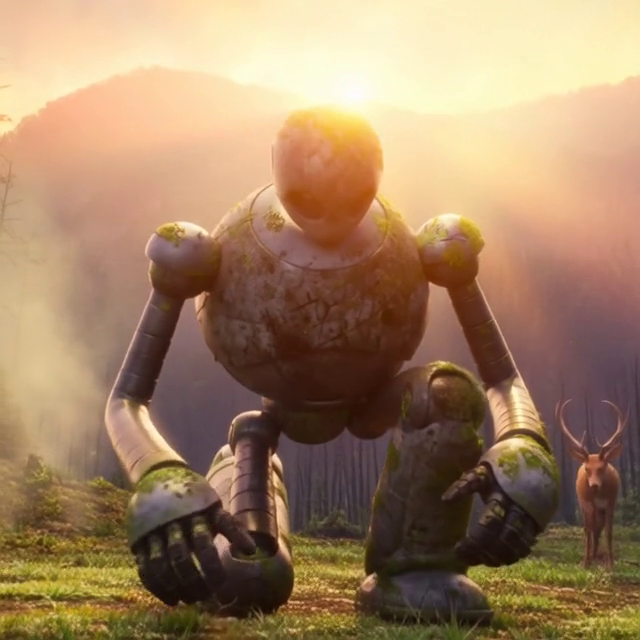
\includegraphics[width=\linewidth]
        {../generated-videos/dataset v2/wil1/wan22_i2v/frame_006.png}
    \end{subfigure}
    ~
    \begin{subfigure}{0.45\columnwidth}
        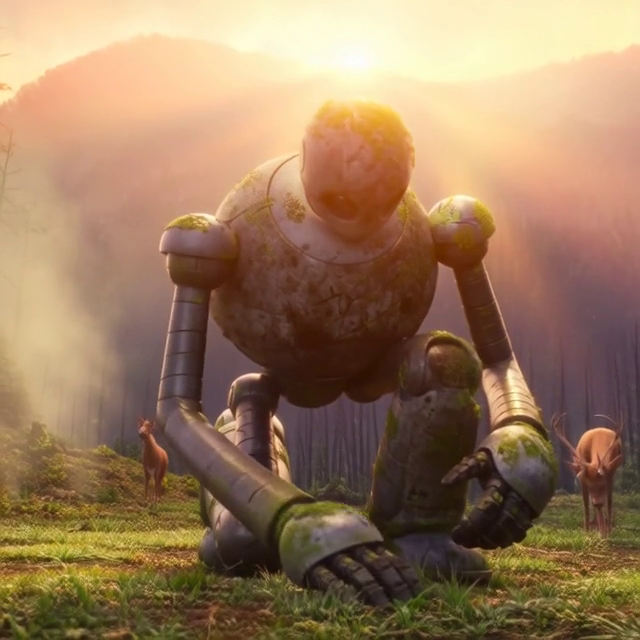
\includegraphics[width=\linewidth]
        {../generated-videos/dataset v2/wil1/wan22_i2v/frame_008.png}
    \end{subfigure}
    \caption{Wan~2.2's extension of \textit{The Wild Robot}}
\end{figure}

Beyond these isolated mechanical tests, we evaluate production readiness
by testing each model's ability to extend a given scene. In the teaser
figure, we provide Wan~2.2~(14B) with a single frame from DreamWorks'
\textit{The Wild Robot} and prompt it to show Roz bending to touch the
grass while a deer roams freely in the background, a task that demands
character identity preservation, physically plausible articulated motion,
and coherent background animation simultaneously.



Our evaluation framework isolates specific mechanical and perceptual
parameters through a curated set of targeted prompts, described in
full in Section~\ref{sec:targeted_and_stress_testing}. The
\textit{Red Cube} prompt (\ref{prompt:1}) evaluates whether a
primitive geometric shape can maintain its absolute structural and color
integrity during smooth, continuous camera translation. The
\textit{Rubber Ball} prompt (\ref{prompt:2}) assesses the
model's understanding of basic Newtonian physics. For multi-step reasoning, the
\textit{Tea Sequence} (\ref{prompt:6}) challenges the model to
link distinct sequential actions into a cohesive narrative timeline
without skipping steps or losing contextual memory. Stylistic
evaluation includes an anime-style cat prompt (\ref{prompt:c}),
designed to probe each model's understanding of Japanese animation
conventions: cel-shading, exaggerated proportions, and the modulation
of perceived frame rates characteristic of limited animation.

The models evaluated in this study are Grok (xAI), Kling O3
(Kuaishou), LTX~2.6 and LTX~2.3 (Lightricks), Seedance~1.5
(ByteDance), Google Veo~3 (DeepMind), Vidu~Q3 (ShengShu), and
Wan~2.2 (Alibaba) \cite{deepmind2024veo, kuaishou2025kling,
    hacohen2026ltx, bytedance2025seedance, xai2025grok, shengshu2024vidu,
    alibaba2025wan}. This selection spans the full spectrum from
resource-constrained open-source models to closed proprietary systems,
allowing direct comparison under equivalent prompting conditions. The
complete prompt list is provided in Appendix~\ref{app:prompts}; the
evaluation parameters are defined in Appendix~\ref{app:parameters};
and all generated video outputs are available on
\href{https://t-cent.github.io/Character-Consistency}{the accompanying
    webpage}.

The remainder of this paper is structured as follows.
Section~\ref{sec:background} surveys the architectural evolution of
generative video models and contextualizes our evaluation methodology
relative to existing benchmarks. Section~\ref{sec:targeted_and_stress_testing}
describes our prompt design and stress-testing methodology.
Section~\ref{sec:evaluation} presents quantitative and qualitative
results across all models and prompts. Section~\ref{sec:architectures}
discusses the architectural backbones of each evaluated model and
connects design choices to the observed performance patterns.

% To summarize, this paper makes the following contributions:
% \begin{itemize}
%     \item A curated set of 13 targeted evaluation prompts designed to 
%     isolate specific mechanical, spatial, temporal, and stylistic 
%     capabilities in T2V models, together with 6 animation style 
%     prompts and 14 production-level stress tests.
%     \item A systematic qualitative and quantitative evaluation of 8 
%     current SOTA generative video models, spanning both open-source 
%     and proprietary systems.
%     \item An image continuation experiment using frames from 
%     professional film productions, evaluating model readiness for 
%     production-adjacent previz workflows.
%     \item An architectural analysis connecting each model's design 
%     choices to its observed failure modes, providing actionable 
%     guidance for practitioners integrating generative video into 
%     professional pipelines.
%     \item A publicly released dataset of all generated videos to 
%     facilitate reproducibility and future benchmarking research.
% \end{itemize}

\section{Background and Related Work}
\label{sec:background}

The landscape of Generative Artificial Intelligence (AI) for video synthesis
has evolved rapidly, transitioning from early exploratory architectures to
massive, data-driven foundation models \cite{kaswan2023generative,
    xie2025comprehensive}. This evolution has been accompanied by a parallel
development in evaluation methodology, as the community has recognized that
simple quantitative metrics are insufficient to capture the full range of
model capabilities and failure modes \cite{huang2024vbench,
    liu2024evalcrafter}. To contextualize the models evaluated in this study,
it is crucial to understand the underlying architectures and how they
generate high-dimensional spatio-temporal data under the hood.

\subsection{Foundational Generative Architectures}
Early approaches to text-to-video (T2V) generation relied predominantly on
Variational Autoencoders (VAEs) and Generative Adversarial Networks (GANs)
\cite{kaswan2023generative, xie2025comprehensive}.
\textbf{VAEs} consist of an encoder that maps input data into a probability
distribution and a decoder that generates new data by sampling from this
learned distribution \cite{xie2025comprehensive}. While structurally simple,
VAEs often suffer from ``posterior collapse'' and struggle to generate highly
complex, high-resolution videos \cite{xie2025comprehensive}.

\begin{figure}[ht]
    \centering
    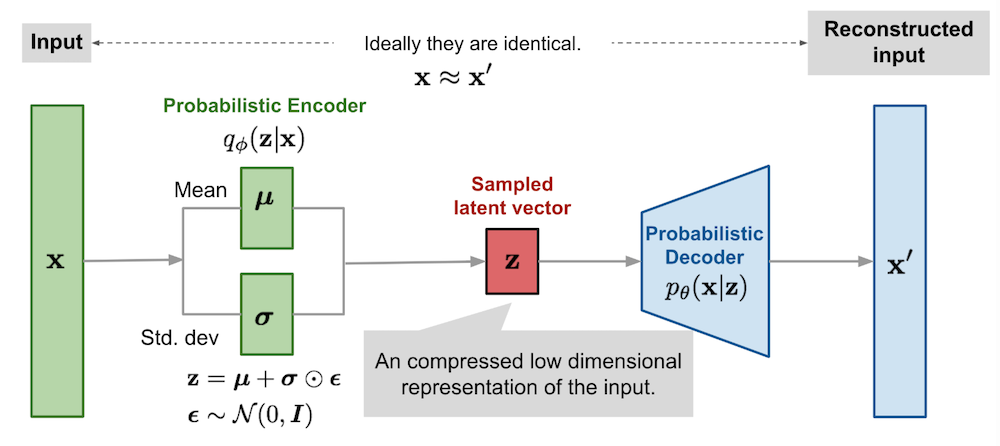
\includegraphics[width=0.7\columnwidth]{images/2026-05-08-17-47-40.png}
    \caption{Variational Autoencoders\protect\footnotemark}
\end{figure}
\footnotetext{Image credit:
    \url{https://yanndubs.github.io/machine-learning-glossary/models/vae}}

\textbf{GANs} operate via an adversarial process between a generator and a
discriminator \cite{xie2025comprehensive}. While capable of producing images
with good perceptual quality, GANs frequently suffer from pattern (mode)
collapse and struggle to scale to complex, large-scale video datasets with
diverse human movements \cite{xie2025comprehensive}.

\begin{figure}[ht]
    \centering
    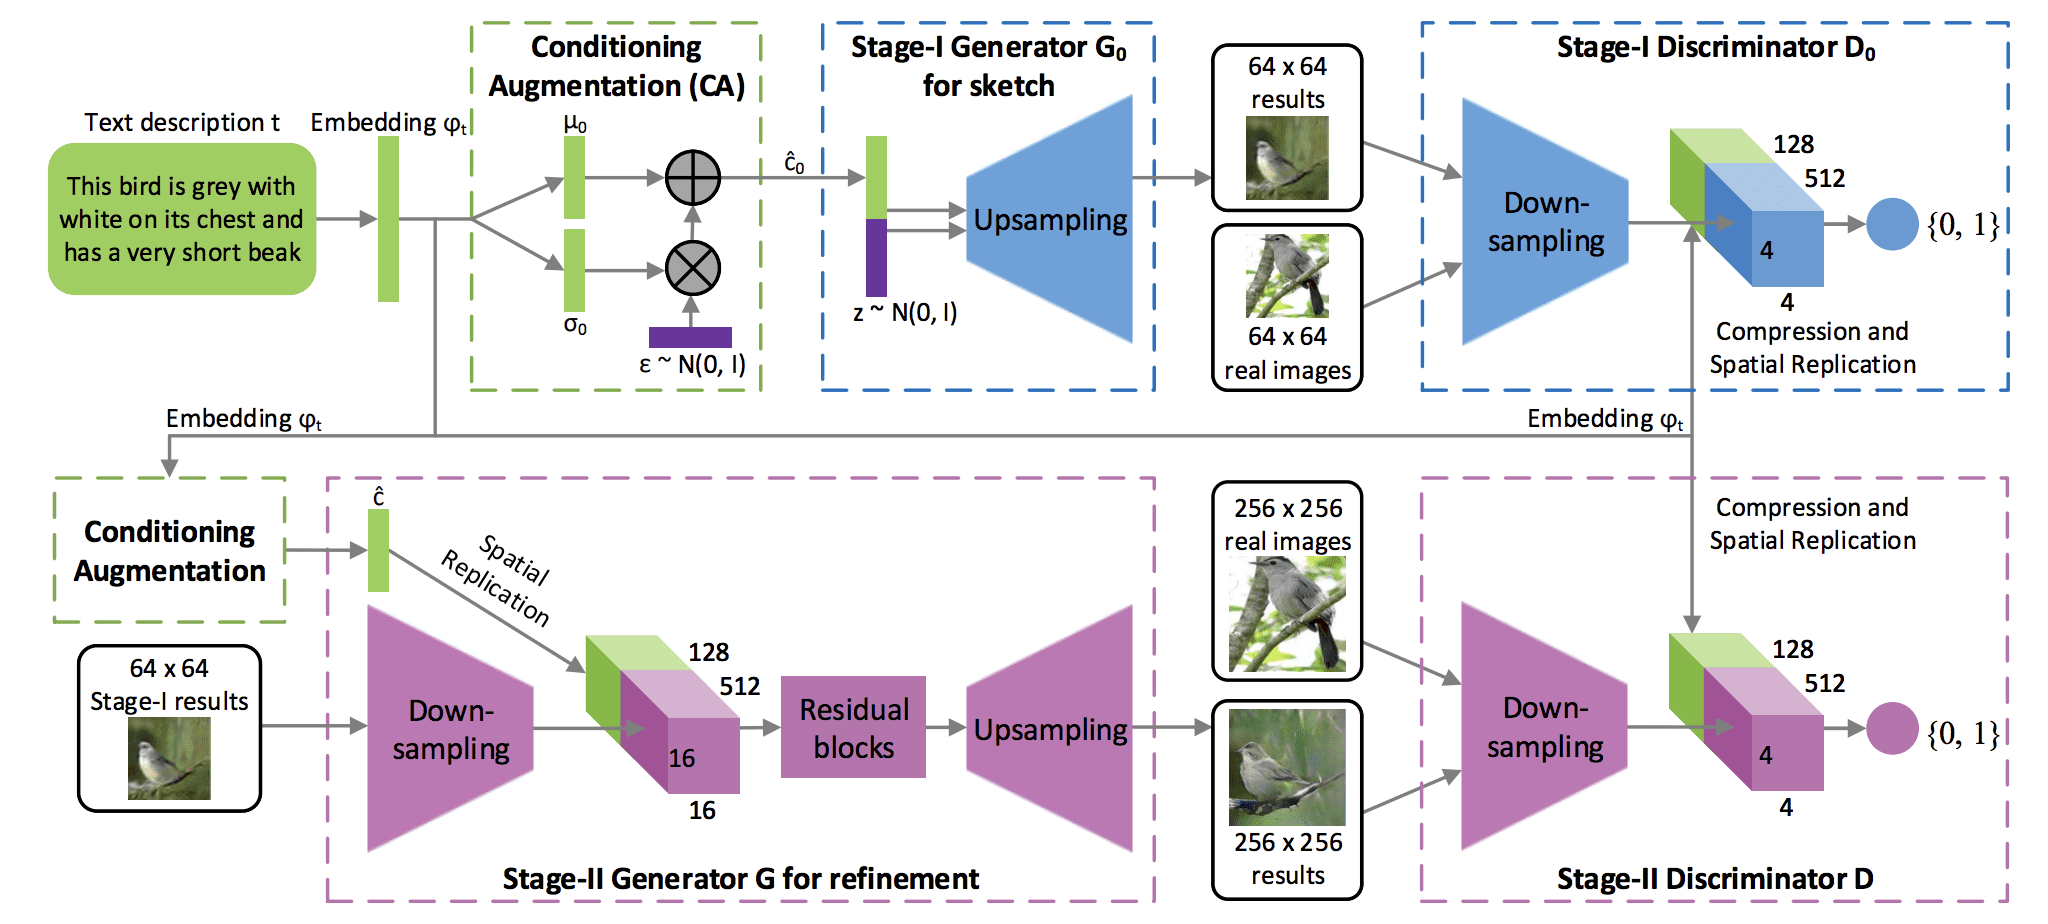
\includegraphics[width=0.7\columnwidth]{images/2026-05-08-18-01-19.png}
    \caption{Generative Adversarial Networks\protect\footnotemark}
\end{figure}
\footnotetext{Image credit:
    \url{https://machinelearningmastery.com/tour-of-generative-adversarial-network-models/}}

To overcome these limitations, the field shifted toward \textbf{Autoregressive
    Transformers}. These models generate video sequences in a step-by-step manner,
where the latest generated content is conditioned on previously generated frames
\cite{xie2025comprehensive}. This natural fit for sequential data avoids GAN
pattern collapse and yields higher video quality, albeit at the cost of massive
computational and memory resources \cite{xie2025comprehensive}. CogVideo
\cite{hong2022cogvideo} was among the first large-scale autoregressive
transformers applied to open-domain text-to-video generation, demonstrating
that pretraining on large corpora of text-video pairs could yield semantically
coherent outputs. However, autoregressive decoding at video resolution remained
prohibitively slow, motivating the subsequent shift to diffusion-based
pipelines.

\subsection{Under the Hood: Diffusion Models and DiT}
The current generation of state-of-the-art commercial models (including the
architectures powering Sora, Veo, Kling, and others evaluated in this paper)
are predominantly built upon \textbf{Diffusion Models} and \textbf{Diffusion
    Transformers (DiT)}.

\begin{figure}[ht]
    \centering
    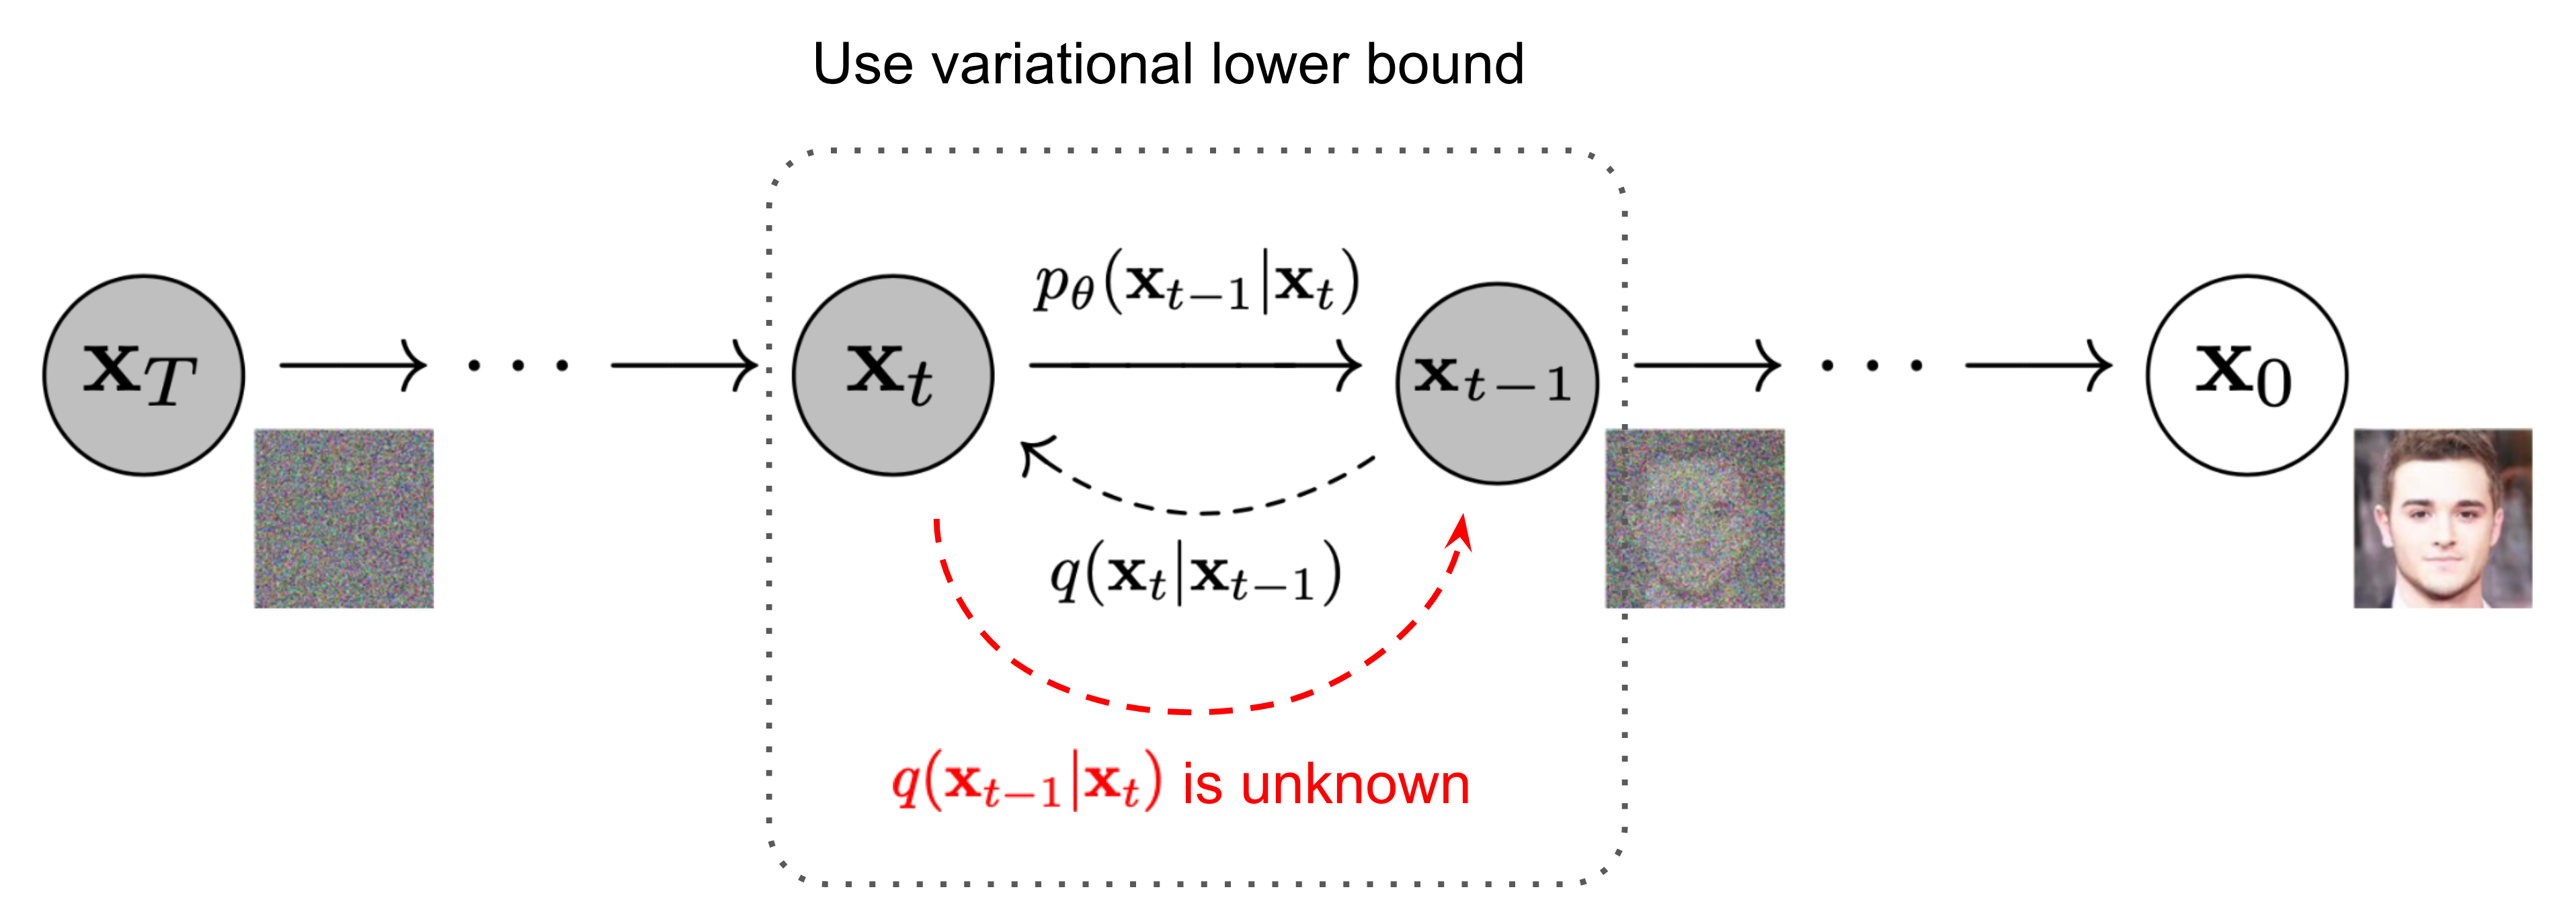
\includegraphics[width=0.7\linewidth]{images/2026-05-08-18-07-51.png}
    \caption{Diffusion models\protect\footnotemark}
\end{figure}
\footnotetext{Image credit:
    \url{https://lilianweng.github.io/posts/2021-07-11-diffusion-models/}}

At its core, a Denoising Diffusion Probabilistic Model (DDPM) learns to
synthesize data by first adding random Gaussian noise to existing data over
a series of steps, and then training a neural network to reverse this process
(denoising) to recover the high-quality image or video \cite{ho2020ddpm}.
Because operating directly in pixel space is computationally prohibitive for
video, modern models utilize \textbf{Latent Diffusion} \cite{rombach2022ldm}.
In this approach, an encoder maps the video into a highly compressed latent
representation, the diffusion process occurs within this smaller latent space,
and a decoder reconstructs the final video pixels, significantly reducing
computational consumption \cite{rombach2022ldm}. Open-source video models such
as VideoCrafter \cite{chen2023videocrafter1} and its successor
VideoCrafter2 \cite{chen2024videocrafter2} demonstrated that this latent
diffusion paradigm could be extended to high-resolution video synthesis,
establishing widely used baselines against which subsequent models are measured.

Recently, the traditional U-Net backbones used in diffusion models have been
replaced by Transformers, creating the \textbf{Diffusion Transformer (DiT)}
architecture \cite{peebles2023dit}. DiT replaces the inductive biases of
convolution with the global attention mechanism of transformers operating
directly on latent patches, and demonstrates that model quality scales
predictably with compute \cite{peebles2023dit}. Models utilizing DiT
(such as OpenAI's Sora \cite{openai2024sora}) exhibit several advanced
capabilities under the hood, such as \textbf{Variable Resolution Training}
which allows the model to be trained natively on videos and images of varying
resolutions, durations, and aspect ratios without extreme cropping
\cite{openai2024sora} and \textbf{Prompt Expansion} which leverages Large
Language Models (LLMs) to automatically convert short, vague user prompts
into highly detailed instructions, drastically improving the semantic
alignment and quality of the generated video \cite{openai2024sora}.
CogVideoX \cite{yang2024cogvideox} extended the DiT framework with an
``expert transformer'' specifically designed for long-duration temporal
coherence, representing the state of the art in open-source DiT-based video
generation at the time of writing.

\subsection{The Necessity of Stress Testing}
\label{sec:stress_necessity}

Traditionally, T2V models are evaluated using automated quantitative metrics
such as Fr\'{e}chet Video Distance (FVD) and Inception Score (IS) for visual
quality, alongside CLIPSIM for text-video semantic alignment
\cite{xie2025comprehensive}.

However, recent studies indicate that these automated evaluation metrics often
misalign with actual human judgments and fail to capture nuanced failures in
temporal consistency, physics, and complex motion \cite{huang2024vbench,
    liu2024evalcrafter}. To address this, the community has proposed increasingly
targeted benchmarks. VBench \cite{huang2024vbench} decomposes video generation
quality into 16 fine-grained dimensions, including subject consistency,
motion smoothness, and spatial relationships, and validates each dimension
against human preference annotations, demonstrating that single-metric
evaluation systematically misrepresents model capabilities. EvalCrafter
\cite{liu2024evalcrafter} similarly proposes 17 objective metrics spanning
visual quality, motion quality, and text-video alignment, finding that
human-aligned composite scoring is significantly more reliable than any
individual automated metric.

Crucially for the present work, VideoPhy \cite{bansal2024videophy} established
that physical commonsense is a distinct and severely underperforming capability
in current T2V models: even the best-performing model evaluated in that study
satisfied physical constraints in fewer than 40\% of generated videos. This
directly motivates several of our stress-testing prompts, including the rubber
ball (\ref{prompt:2}), glass slide (\ref{prompt:7}), and the
multi-stage stress tests in Section~\ref{sec:targeted_and_stress_testing}. T2V-CompBench
\cite{sun2024t2vcompbench} further demonstrated that compositional generation (coordinating multiple objects, their attributes, and spatial relationships
simultaneously) remains an open challenge, directly motivating our
multi-agent coordination (\ref{prompt:8}) and spatial geometry
(\ref{prompt:11}) evaluations.

Taken together, this body of work establishes that qualitative, human-centered,
and capability-targeted evaluation is not merely complementary to automated
metrics but is essential for understanding the production readiness of T2V
systems. Our methodology builds on this insight by constructing a curated set
of stress-testing prompts designed to isolate specific mechanical, spatial,
temporal, and stylistic capabilities, and by evaluating models that represent
the current commercial frontier — several of which postdate existing benchmarks
entirely.

\section{Targeted Prompts and Stress Testing Methodology}
\label{sec:targeted_and_stress_testing}
To isolate specific failure modes and evaluate foundational capabilities, we utilize our set of targeted prompts designed to test specific domains as listed in Appendix~\ref{app:parameters}.
This provides a neutral baseline before introducing complex, multi-layered scenarios as mentioned in Section~\ref{sec:stress_prompts} and Section~\ref{sec:image_continuation}.

\subsection{Dataset Creation}

We briefly describe our generation pipeline and prompts used. ComfyUI on a Windows machine using a single NVIDIA 4080 SUPER was used for generation of all videos with the default seeds and parameters. In each of the following section, we first describe how our prompts achieves its baseline test and we then display randomly sampled frames from four such generated videos for select prompts. Additional material may be viewed from the complete dataset.


\subsection{Targeted Prompts: Metric Baselines}



\ref{prompt:1} (red cube) testing temporal consistency \ref{param:1}. Evaluates whether a primitive geometric shape can maintain its absolute structural and color integrity during continuous, smooth camera translation without morphing or flickering.

\displayimages{Grok}{kling\_o3\_t2v}{ltx-t2v}{seedance}{1}{Grok}{Kling}{LTX}{Seedance}


\ref{prompt:2} (rubber ball) testing motion realism \ref{param:2}, objection interaction \& physics reasoning \ref{param:7}. Assesses the model's understanding of basic Newtonian physics, specifically gravity, elasticity, momentum preservation, and kinetic energy decay upon contact with a rigid surface.

\displayimages{veo}{kling\_o3\_t2v}{ltx-t2v}{seedance}{2}{Google Veo}{Kling}{LTX}{Seedance}


\ref{prompt:3} (wooden chair) testing camera behavior \ref{param:3}. Evaluates whether the model can execute a stable and physically plausible forward dolly movement without introducing camera shake, spatial distortion, temporal jitter, or discontinuities in perspective projection.

\displaylocalimages{21}{3}

\ref{prompt:4} (white sphere) testing lighting stability \ref{param:4}. Assesses whether illumination, surface shading gradients, and cast shadows remain temporally coherent under static scene conditions without flickering, drifting, or inconsistent light transport artifacts.

\displaylocalimages{22}{4}

\ref{prompt:5} (green shirt) testing character preservation \ref{param:5}. Evaluates whether anatomical structure, clothing appearance, body proportions, and identity-specific visual features remain temporally stable throughout continuous locomotion without morphing or feature drift.

\displaylocalimages{23}{5}

\ref{prompt:6} (cup of tea) testing prompt inference and context \ref{param:6}, long-horizon coherence \ref{param:10}. Assesses the model's ability to maintain causal narrative sequencing across multiple sequential actions while preserving contextual memory and temporal continuity over an extended action chain.

\displayimages{vidu\_q3\_t2v}{veo}{ltx-t2v}{seedance}{3}{Vidu}{Google Veo}{LTX}{Seedance}


\ref{prompt:7} (glass slide) testing object interaction \& physics reasoning \ref{param:7}. Evaluates whether the model correctly simulates force transfer, frictional deceleration, inertial motion, and contact dynamics between an articulated agent and a rigid body object.


\ref{prompt:8} (red, green, blue) testing multi-agent coordination \ref{param:8}, temporal consistency \ref{param:1}. Assesses the ability to independently preserve identity, motion synchronization, and spatial separation across multiple simultaneously moving entities without merging, color bleeding, or inconsistent velocity behavior.

\begin{figure}[H]
    \centering

    % Top row — LTX
    \begin{subfigure}{0.45\columnwidth}
        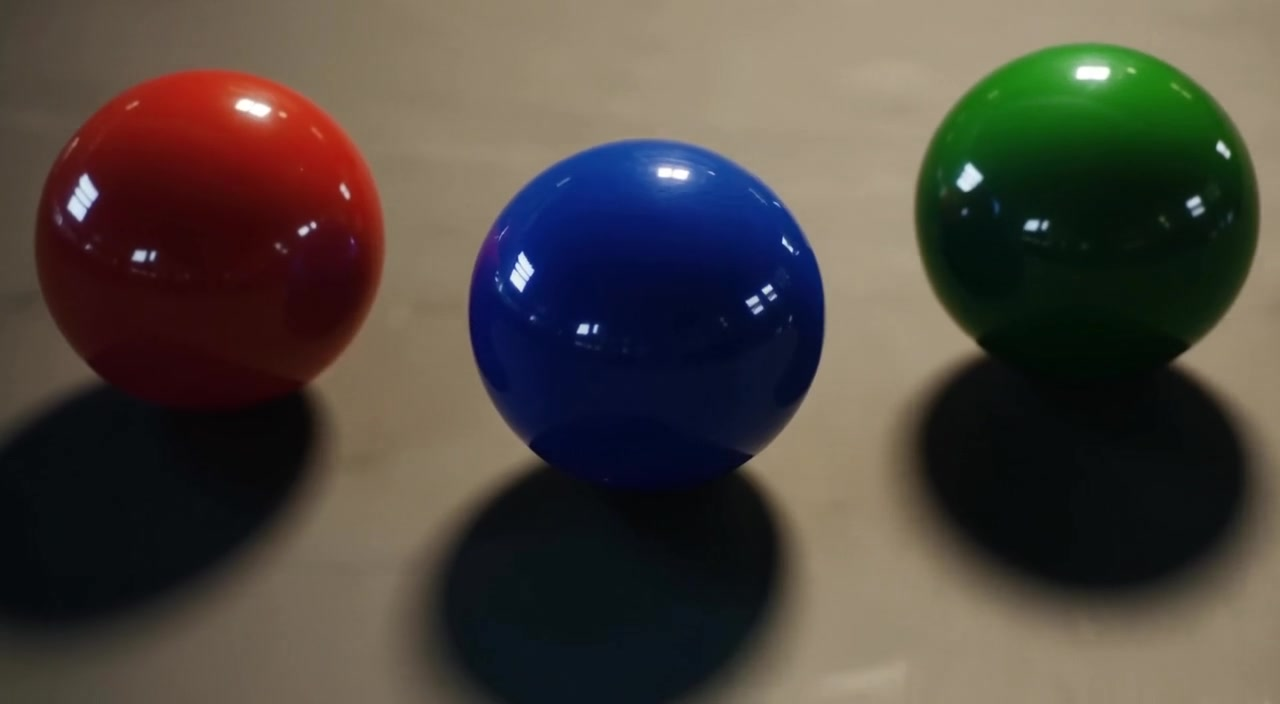
\includegraphics[width=\linewidth]{../generated-videos/local/frames/LTX_2.3_t2v_00015_/LTX_2.3_t2v_00015__01.jpg}
    \end{subfigure}
    ~
    \begin{subfigure}{0.45\columnwidth}
        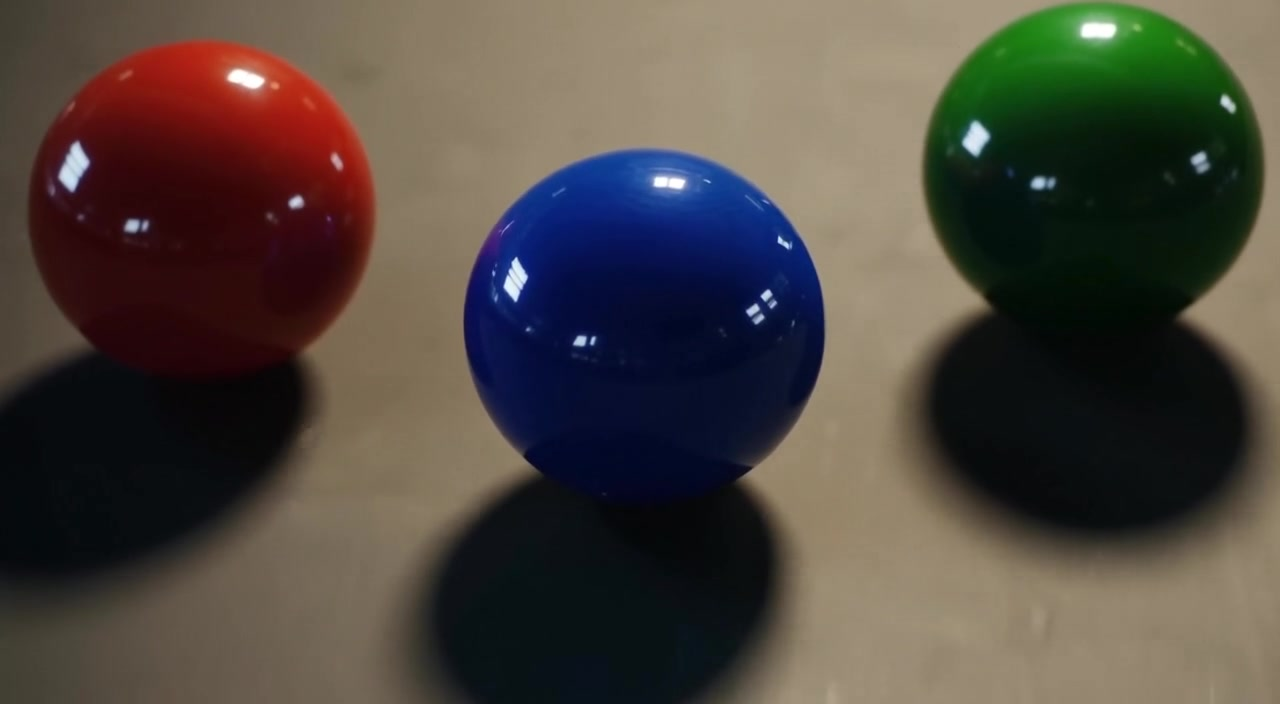
\includegraphics[width=\linewidth]{../generated-videos/local/frames/LTX_2.3_t2v_00015_/LTX_2.3_t2v_00015__04.jpg}
    \end{subfigure}

    \vspace{0.5em}

    \caption*{LTX 2.3}

    \vspace{1em}

    % Bottom row — Wan
    \begin{subfigure}{0.45\columnwidth}
        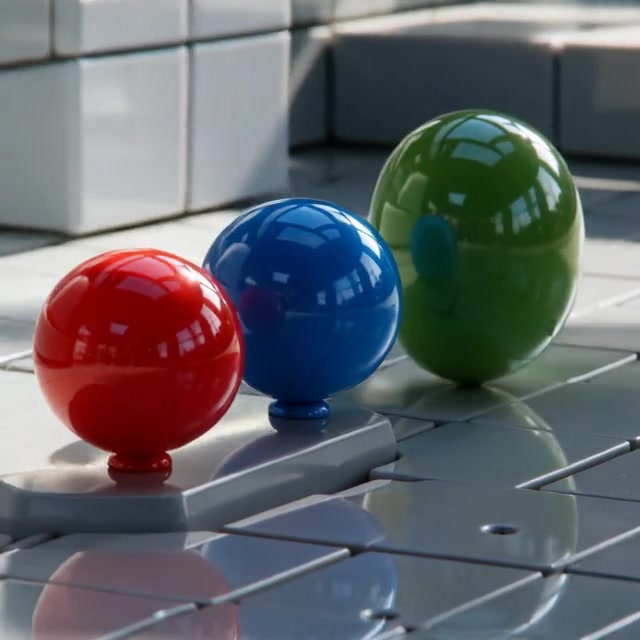
\includegraphics[width=\linewidth]{../generated-videos/local/frames/ComfyUI_00033_/ComfyUI_00033__01.jpg}
    \end{subfigure}
    ~
    \begin{subfigure}{0.45\columnwidth}
        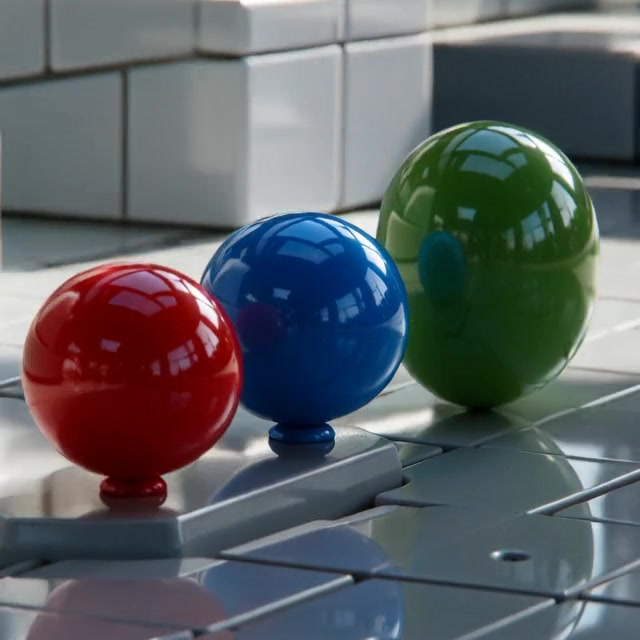
\includegraphics[width=\linewidth]{../generated-videos/local/frames/ComfyUI_00033_/ComfyUI_00033__04.jpg}
    \end{subfigure}

    \vspace{0.5em}

    \caption*{Wan 2.2 (14B)}

\end{figure}

\ref{prompt:9} (large box) testing spatial reasoning \& geometry \ref{param:12}, character preservation \ref{param:5}. Evaluates object permanence, occlusion reasoning, and trajectory continuity by determining whether the model preserves subject identity and spatial consistency while the character is temporarily hidden from view.

\begin{figure}[H]
    \centering

    % Top row — LTX
    \begin{subfigure}{0.45\columnwidth}
        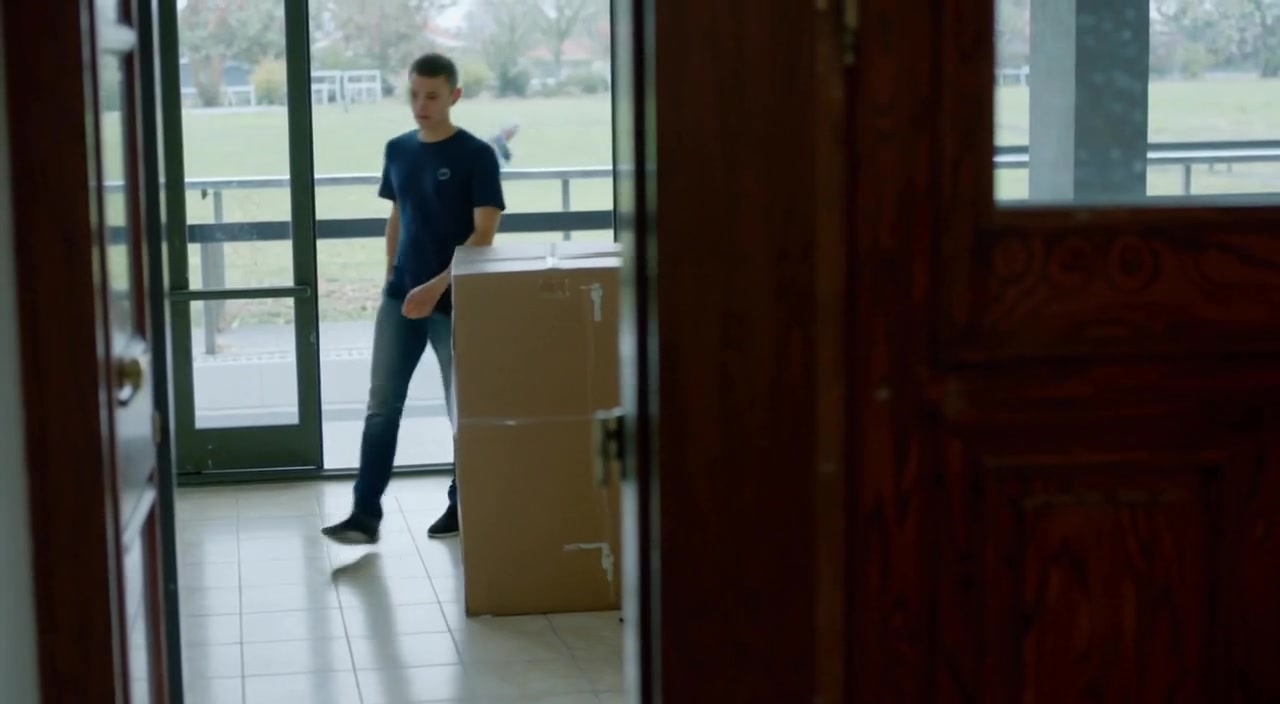
\includegraphics[width=\linewidth]{../generated-videos/local/frames/LTX_2.3_t2v_00013_/LTX_2.3_t2v_00013__01.jpg}
    \end{subfigure}
    ~
    \begin{subfigure}{0.45\columnwidth}
        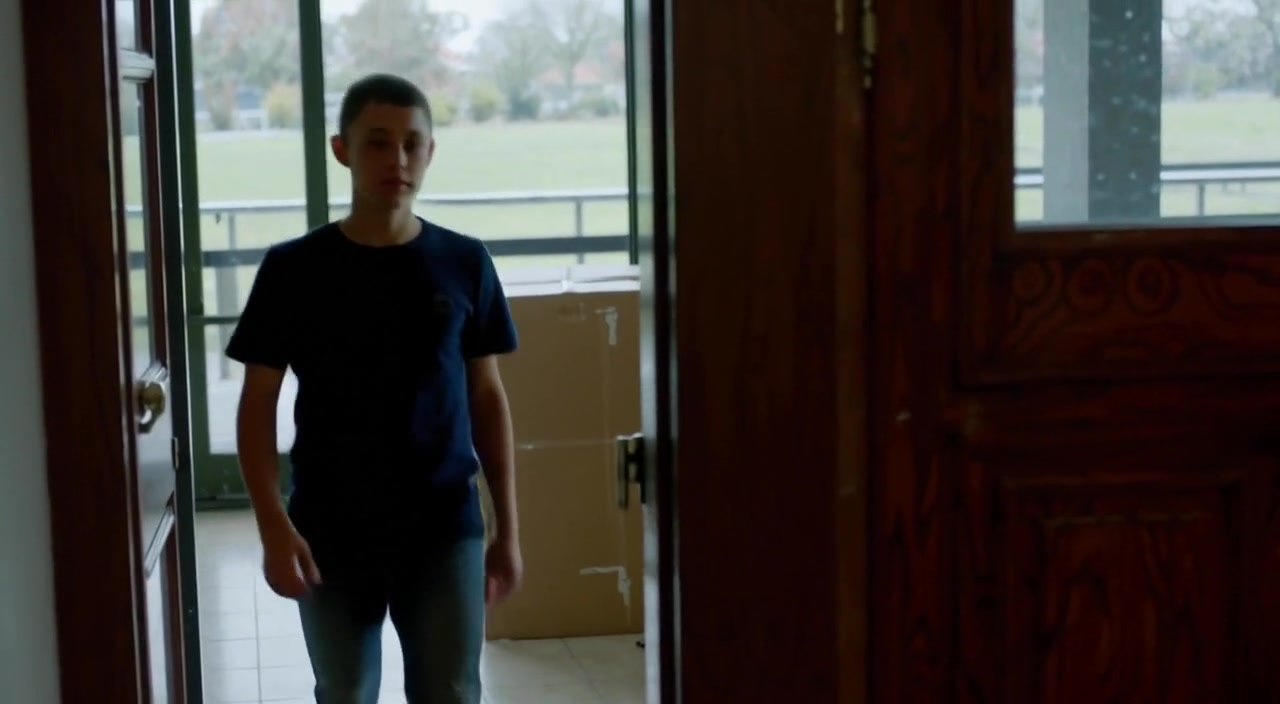
\includegraphics[width=\linewidth]{../generated-videos/local/frames/LTX_2.3_t2v_00013_/LTX_2.3_t2v_00013__04.jpg}
    \end{subfigure}

    \vspace{0.5em}

    \caption*{LTX 2.3}

    \vspace{1em}

    % Bottom row — Wan
    \begin{subfigure}{0.45\columnwidth}
        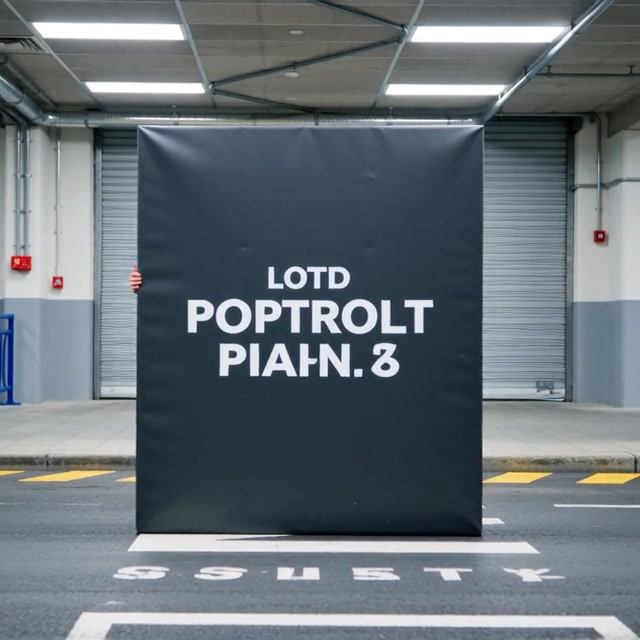
\includegraphics[width=\linewidth]{../generated-videos/local/frames/ComfyUI_00031_/ComfyUI_00031__01.jpg}
    \end{subfigure}
    ~
    \begin{subfigure}{0.45\columnwidth}
        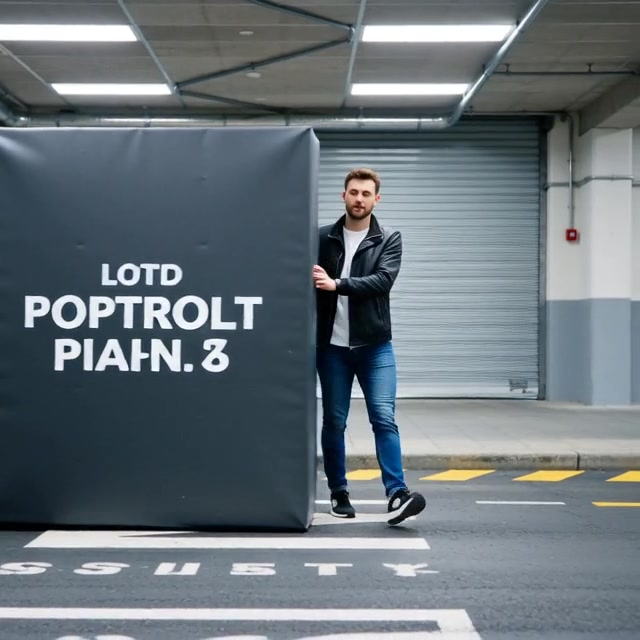
\includegraphics[width=\linewidth]{../generated-videos/local/frames/ComfyUI_00031_/ComfyUI_00031__04.jpg}
    \end{subfigure}

    \vspace{0.5em}

    \caption*{Wan 2.2 (14B)}

\end{figure}

\ref{prompt:10} (striped shirt) testing fine-grained detail consistency \ref{param:9}, camera behavior \ref{param:3}. Assesses whether high-frequency texture details remain stable during continuous zoom motion without introducing aliasing, texture swimming, moir\'{e} artifacts, or geometric distortion.

\displayimages{Grok}{kling\_o3\_t2v}{ltx-t2v}{seedance}{4}{Grok}{Kling}{LTX}{Seedance}


\ref{prompt:11} (cube and sphere) testing spatial reasoning \& geometry \ref{param:12}. Evaluates whether the model preserves correct depth relationships, parallax behavior, and relative object positioning during lateral camera translation in a 3D spatial configuration.


\ref{prompt:12} (OPEN) testing text rendering \ref{param:13}. Assesses whether typographic structures remain geometrically stable and semantically legible during camera motion without character deformation, symbol substitution, or temporal instability in fine textual details.

\subsection{Targeted Prompts: Animation Styles}

\ref{prompt:a} (base cat walk). Establishes the model's default visual prior by evaluating its unprompted choices for lighting, texture fidelity, scene composition, and motion representation in the absence of explicit stylistic conditioning.

\displayimages{Grok}{kling\_o3\_t2v}{ltx-t2v}{seedance}{5}{Grok}{Kling}{LTX}{Seedance}


\ref{prompt:b} (cartoon-style cat). Assesses adherence to stylized western animation aesthetics, including simplified geometry, controlled shape language, clean contour definition, reduced material realism, and intentionally abstracted motion behavior.

\displayimages{Grok}{kling\_o3\_t2v}{ltx-t2v}{seedance}{7}{Grok}{Kling}{LTX}{Seedance}


\ref{prompt:c} (anime-style cat). Evaluates the model's understanding of anime-specific visual conventions such as exaggerated proportions, cel-shading behavior, stylized facial structure, limited-animation aesthetics, and temporally coherent stylized motion.


\begin{figure}[H]
    \centering

    % Top row — LTX
    \begin{subfigure}{0.45\columnwidth}
        
\includegraphics[width=\linewidth]{../generated-videos/local/frames/LTX_2.3_t2v_00009_/LTX_2.3_t2v_00009__01.jpg}
    \end{subfigure}
    ~
    \begin{subfigure}{0.45\columnwidth}
        
\includegraphics[width=\linewidth]{../generated-videos/local/frames/LTX_2.3_t2v_00009_/LTX_2.3_t2v_00009__04.jpg}
    \end{subfigure}

    \vspace{0.5em}

    \caption*{LTX 2.3}

    \vspace{1em}

    % Bottom row — Wan
    \begin{subfigure}{0.45\columnwidth}
        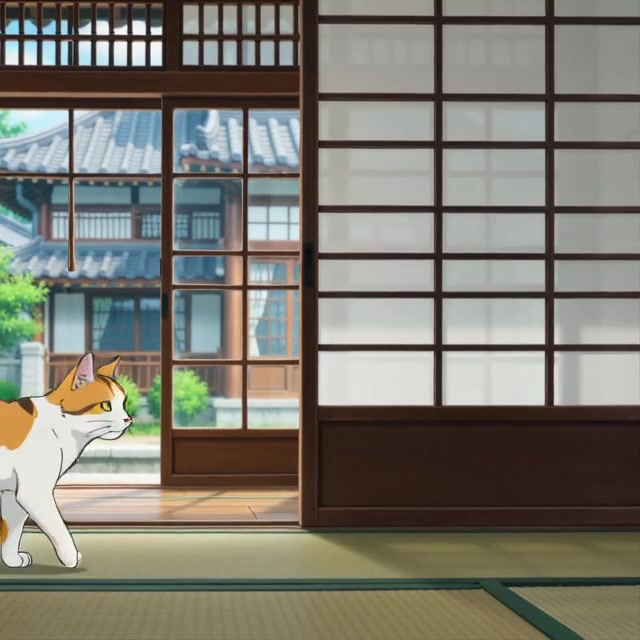
\includegraphics[width=\linewidth]{../generated-videos/local/frames/ComfyUI_00027_/ComfyUI_00027__01.jpg}
    \end{subfigure}
    ~
    \begin{subfigure}{0.45\columnwidth}
        
\includegraphics[width=\linewidth]{../generated-videos/local/frames/ComfyUI_00027_/ComfyUI_00027__04.jpg}
    \end{subfigure}

    \vspace{0.5em}

    \caption*{Wan 2.2 (14B)}

\end{figure}


\ref{prompt:d} (realistic cat). Assesses the ability to synthesize believable organic textures, physically plausible lighting, natural environmental shading, and realistic quadrupedal locomotion consistent with cinematic rendering conventions.

\begin{figure}[H]
    \centering

    % Top row — LTX
    \begin{subfigure}{0.45\columnwidth}
        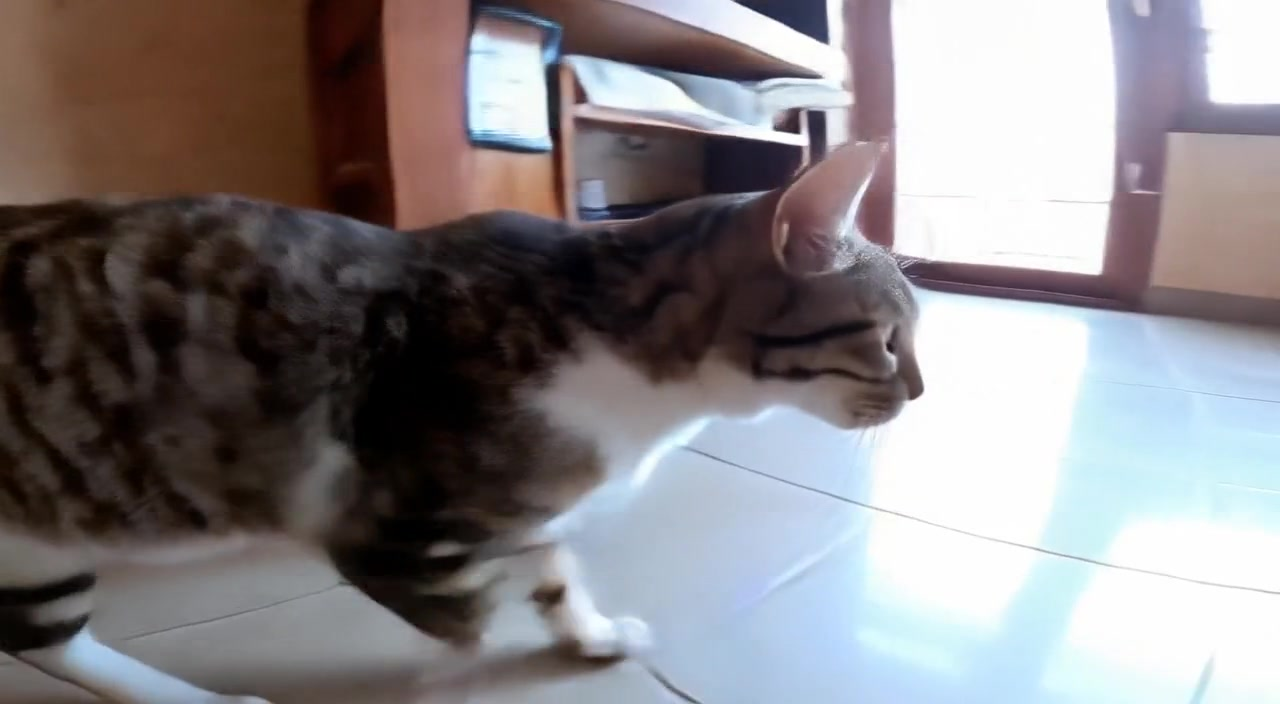
\includegraphics[width=\linewidth]{../generated-videos/local/frames/LTX_2.3_t2v_00010_/LTX_2.3_t2v_00010__01.jpg}
    \end{subfigure}
    ~
    \begin{subfigure}{0.45\columnwidth}
        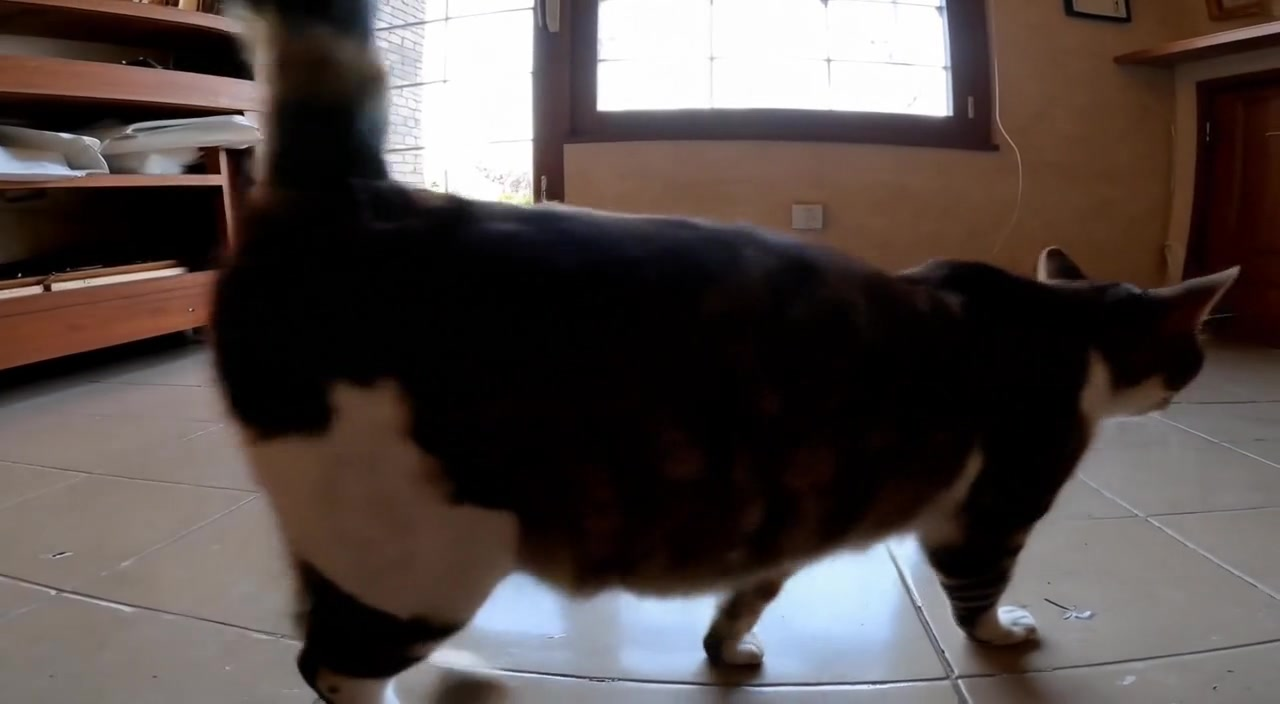
\includegraphics[width=\linewidth]{../generated-videos/local/frames/LTX_2.3_t2v_00010_/LTX_2.3_t2v_00010__04.jpg}
    \end{subfigure}

    \vspace{0.5em}

    \caption*{LTX 2.3}

    \vspace{1em}

    % Bottom row — Wan
    \begin{subfigure}{0.45\columnwidth}
        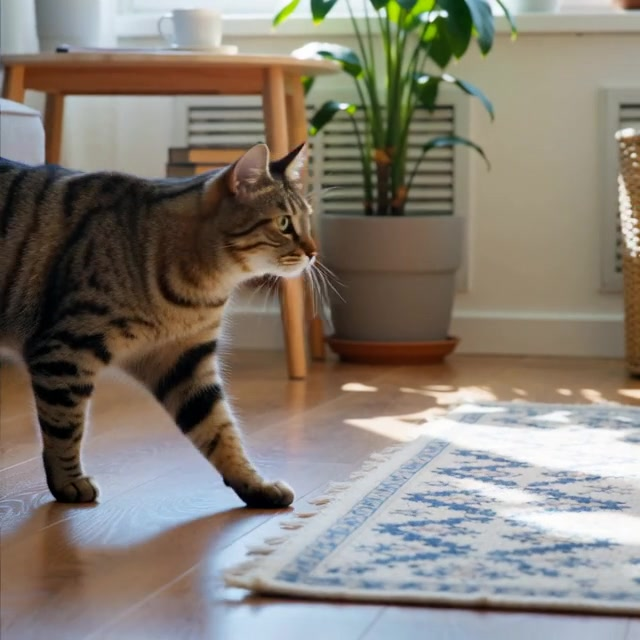
\includegraphics[width=\linewidth]{../generated-videos/local/frames/ComfyUI_00028_/ComfyUI_00028__01.jpg}
    \end{subfigure}
    ~
    \begin{subfigure}{0.45\columnwidth}
        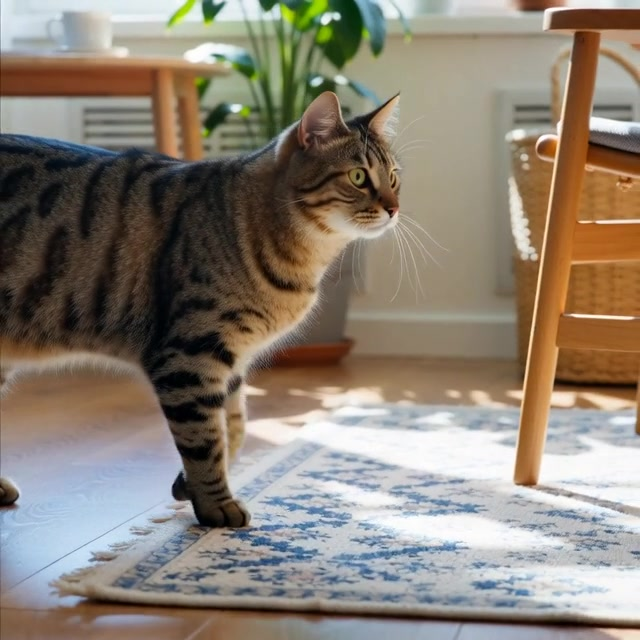
\includegraphics[width=\linewidth]{../generated-videos/local/frames/ComfyUI_00028_/ComfyUI_00028__04.jpg}
    \end{subfigure}

    \vspace{0.5em}

    \caption*{Wan 2.2 (14B)}

\end{figure}


\ref{prompt:e} (photo-realistic cat). Evaluates high-fidelity rendering capability through micro-texture preservation, advanced material realism, complex indirect lighting behavior, realistic fur dynamics, and image statistics closely matching physical camera capture.

\displayimages{Grok}{kling\_o3\_t2v}{ltx-t2v}{veo}{6}{Grok}{Kling}{LTX}{Veo}


\ref{prompt:f} (educational-style animation). Assesses whether the model can intentionally simplify visual presentation for instructional clarity while preserving semantic readability, motion intelligibility, and diagrammatic communication structure typical of educational media.

\subsection{Stress Testing Prompts}
\label{sec:stress_prompts}
These prompts combine multiple domains to test the limits of model coherence across extended durations and complex interactions, serving as practical production-level evaluations. The results help filmmakers assess the degree of creative and post-production control possible with generative AI, while also emphasizing locally run models for privacy and intellectual property protection. Every frame that follows is generated by LTX 2.3.


% \begin{itemize}
%     \item \textbf{Stress Test 1:} ``A person prepares a cup of tea from start to finish: boiling water, pouring it into a cup, adding a tea bag, and letting it steep. The sequence is continuous and logically consistent.''
%           \\ \textbf{Testing:} Long-horizon coherence [10], Object interaction \& physics reasoning [7], Prompt inference [6].
%           \\ \textbf{How:} A severe test of sequential logic and state changes. It requires the model to track liquid physics, precise tool manipulation, and material changes (water turning brown) over an extended timeframe without temporal degradation.

%     \item \textbf{Stress Test 2:} ``Two people sit across from each other at a table and pass a book back and forth. The interaction is smooth and coordinated.''
%           \\ \textbf{Testing:} Multi-agent coordination [8], Object interaction \& physics reasoning [7].
%           \\ \textbf{How:} Evaluates synchronized interaction between multiple human subjects and a shared prop. It tests spatial geometry to ensure hands align perfectly with the object during hand-offs without clipping or floating.

%     \item \textbf{Stress Test 3:} ``A busy street scene where cars move in one direction while pedestrians walk on the sidewalk. No objects collide, and motion remains consistent.''
%           \\ \textbf{Testing:} Multi-agent coordination [8], Spatial reasoning \& geometry [12], Long-horizon coherence [10].
%           \\ \textbf{How:} A high-density environmental test. It evaluates the model's ability to independently track dozens of distinct entities moving in parallel trajectories (cars vs.\ pedestrians) without cross-contamination, logic failures, or sudden disappearances over time.
% \end{itemize}

\begin{enumerate}[label=\textbf{Stress Test \arabic*}, leftmargin=*]

    \item
          A huge, muscular man jumps between narrow rooftops, landing hard, rolling, and immediately sprinting forward; muscles flex, skin compresses, and hair and clothing react naturally to motion.

          \displaycontinuousimages{5}{Impressive environment; incorrect scale}

    \item
          Godzilla stands on a suspension bridge as a fully loaded cargo ship crashes into the supports; cables snap, the bridge bends, and debris falls into the water below.

          \displaycontinuousimages{6}{No physical interactions; incorrect scale}


          % \item
          % Doctor Strange wearing a blue coat fights an identical doppelgänger mid-air, exchanging spells while crashing through multiple buildings; faces, costumes, and body proportions remain consistent throughout.

    \item
          A doctor studies a close-up chest X-ray showing multiple dark spots, then turns to discuss the findings in a softly lit hospital room filled with medical equipment.

          \displaycontinuousimages{7}{Impressive realism; gibberish text}


    \item
          An extreme close-up of a human eye blinking slowly; eyelashes bend, tear fluid shifts, and reflections in the cornea subtly move.

          \displaycontinuousimages{8}{Extremely realistic}


    \item
          A handheld camera follows a cyclist through a crowded market street, weaving between people and stalls, with occasional motion blur and focus shifts.

          \displaycontinuousimages{9}{Convincing environment; no collision}


    \item
          An abstract microscopic view of protozoa swimming in fluid, flagella waving, bodies deforming as they collide and consume smaller organisms.

          \displaycontinuousimages{3}{Convinicing animation; replaced protozoa with fish}


    \item
          A medical simulation showing how poison spreads from a snake bite on a wrist, flowing through veins over time with semi-transparent anatomical layers.

    \item
          A red ball rolls behind a couch, briefly disappears, then re-emerges on the other side without changing color, shape, or size.

          \displaycontinuousimages{4}{Incorrect side of couch}


    \item
          A brick wall seen up close as the camera slowly pans sideways; mortar lines and brick patterns remain stable without warping.

    \item
          Five people play basketball, passing the ball, setting screens, colliding lightly, and reacting naturally to each other's movements.
          \displaycontinuousimages{2}{Multiple basketballs at once}

    \item
          A man places his keys on a table, leaves the room, returns later, and picks up the same keys from the same spot.

    \item
          A hand-painted watercolor-style fox runs through a forest; the painterly texture stays consistent while motion remains smooth and believable.

    \item
          A realistic car slowly transforms into a humanoid robot, with mechanical parts unfolding logically and no sudden shape popping.

\end{enumerate}

\subsection{Image Continuation}
\label{sec:image_continuation}

\subsubsection*{Motivation and Ethical Framing}

We continue our testing for production readiness by analyzing the outputs
generated when extending frames from famous films. This experiment is
conducted strictly for academic research purposes, with the intent of
understanding the \textit{capabilities and failure modes} of current
generative video models in a production-adjacent context. We wish to
emphasize unequivocally that \textbf{this work does not advocate for,
    endorse, or facilitate the replacement of directors, cinematographers,
    visual effects artists, animators, or any other creative professionals}
whose artistry is represented in the source material used here. The films
referenced are the creative and intellectual property of their respective
studios and filmmakers; their use here falls within the bounds of academic
fair use for the purposes of commentary, criticism, and research
\cite{usc2011fairuse}.

The specific films referenced in this section are:
\begin{itemize}
    \item \textit{Guillermo del Toro's Pinocchio} (2022), directed by
          Guillermo del Toro and Mark Gustafson, produced by Netflix Animation
          and Double Dare You Productions. All rights reserved by Netflix, Inc.
    \item \textit{WALL-E} (2008), directed by Andrew Stanton, produced
          by Pixar Animation Studios. All rights reserved by The Walt Disney
          Company.
    \item \textit{Pacific Rim} (2013), directed by Guillermo del Toro,
          produced by Legendary Pictures. All rights reserved by Warner Bros.
          Entertainment Inc.
    \item \textit{Southpaw} (2015), directed by Antoine Fuqua, produced
          by Escape Artists and Riche Productions. All rights reserved by
          The Weinstein Company.
\end{itemize}

We selected these four films deliberately to span a range of visual
styles: stop-motion animation, CGI, live-action with heavy visual
effects, and naturalistic live-action drama, so as to probe the
model's generalization across fundamentally different rendering
paradigms. In each case, the first image (top-left) is the original
input frame from the film; the remaining frames are generated
continuations produced by Wan~2.2~(14B).\footnote{The prompts used
    for these experiments are available on
    \href{https://t-cent.github.io/Character-Consistency/list-of-prompts.html\#image-to-video}{our
        webpage}.} The goal is not to reproduce or redistribute the original
creative works but to use single frames as conditioning signals, the
minimal input necessary to test image-to-video continuation fidelity
in a production context.

The broader implication of this experiment for the film industry is not
replacement but \textit{tooling}: understanding where these models
succeed and fail helps production studios make informed decisions about
which pre-production tasks (e.g., rapid storyboard animation,
previz shot extension) might benefit from AI assistance.

% -----------------------------------------------------------------------
\subsubsection*{Guillermo del Toro's \textit{Pinocchio} (2022)}
% -----------------------------------------------------------------------

\displaycontinuousimagesloc{pin2}{Understood elongated nose; incorrect eyes}

\noindent Guillermo del Toro's \textit{Pinocchio} presents an
immediately challenging test case: the film's stop-motion aesthetic
features highly stylized, hand-crafted puppet geometry that deviates
significantly from any photorealistic prior in the model's training
distribution. Notably, Wan~2.2 demonstrates a partial but meaningful
understanding of the source material's most iconic visual feature:
Pinocchio's elongated wooden nose is preserved across generated frames
with reasonable geometric consistency, suggesting that the model has
internalized the character's silhouette from its training data or
correctly infers the nose's rigidity from the input frame's depth cues.

However, the continuation fails on a more subtle but critically
important feature: the eyes. Del Toro's Pinocchio is distinguished by
its expressive, hand-crafted button eyes: wide, asymmetric, and
deliberately wooden in texture. In the generated continuation, the
model substitutes these with anatomically conventional eyes more
consistent with its photorealistic prior, effectively
\textit{de-stylizing} the character. This failure mode is architecturally
consistent with what we observed in Prompt~\textbf{[B]} and
Prompt~\textbf{[C]}: the model's latent space exerts a strong pull
toward realism for facial features specifically, overriding stylistic
conditioning signals when the requested style deviates sufficiently
from photographic norms. For production use, this implies that
AI-assisted continuation of stylized animation would require significant
fine-tuning or LoRA adaptation on the specific visual language of
the target film before it could be trusted even for previsualization.

% -----------------------------------------------------------------------
\subsubsection*{PIXAR's \textit{WALL-E} (2008)}
% -----------------------------------------------------------------------

\displaycontinuousimagesloc{wal1}{Unable to solve the cube}

\noindent \textit{WALL-E} tests a different capability: the model's
ability to continue a scene in which a mechanically precise,
well-defined 3D object (here, the Rubik's cube) is the focal point of
the action. The input frame depicts WALL-E holding the cube, and
the prompt requests that he attempt to solve it. This is a
demanding test of both character fidelity and \textit{task-directed
    physical reasoning}: a correct continuation would require the model
to simulate plausible cube manipulations (rotating faces, tracking
colored tile positions across frames) while simultaneously preserving
WALL-E's distinctive mechanical design.

The model largely succeeds on the character fidelity axis:
WALL-E's binocular eyes, tracked body, and distinctive color palette
remain consistent across the generated frames, a non-trivial
achievement given the complexity of his geometry. This is consistent
with Wan~2.2's strong performance on character preservation tasks
in the baseline evaluation. However, it completely fails the task
requirement: the Rubik's cube is never manipulated in any physically
meaningful way. Rather than rotating faces, the model produces
subtle surface-level texture drift that superficially resembles
motion but encodes no semantically coherent cube state transitions.
This is a direct manifestation of the long-horizon coherence failure
mode identified in \ref{prompt:6}: the model cannot maintain
a persistent object state (the cube's face configuration) across
frames while simultaneously generating character motion.

% -----------------------------------------------------------------------
\subsubsection*{\textit{Pacific Rim} (2013)}
% -----------------------------------------------------------------------

\displaycontinuousimagesloc{rim1}{Jaeger falls and walks at the same time}

\noindent \textit{Pacific Rim} represents the most technically
demanding test case in this section. The source frame depicts Gypsy Danger, a
Jaeger (a massive, mechanically complex humanoid robot) in a
scene that requires the model to simultaneously maintain the
structural integrity of a highly detailed hard-surface object,
simulate physically plausible bipedal locomotion at an extreme scale,
and preserve the film's distinctive industrial visual language.
The result is a catastrophic failure on multiple simultaneous axes.

Most strikingly, the model \textit{hallucinates a paradoxical
    physical state}: the Jaeger appears to be both falling and walking
at the same time across different portions of the generated
sequence. This is a particularly revealing failure because it
demonstrates that the model has no unified physical state
representation for the subject — different regions of the frame
are being generated with inconsistent motion vectors, producing
a result that is locally plausible (a foot appears to be
stepping; a torso appears to be toppling) but globally
incoherent. This is consistent with the object mitosis failure
observed in \ref{prompt:2} and the multi-agent coordination
failures in \ref{prompt:8}: the model's latent space does
not enforce global physical consistency constraints across the
spatial extent of a single large object.

The scale of the Jaeger also exposes a known weakness in diffusion
models: objects that occupy the majority of the frame at unusual
scales are underrepresented in training data, causing the model to
fall back on statistically common motion priors (e.g., human-scale
walking) that are geometrically incompatible with the subject's
true proportions.

% -----------------------------------------------------------------------
\subsubsection*{\textit{Southpaw} (2015)}
% -----------------------------------------------------------------------

\displaycontinuousimagesloc{paw2}{Impressive continuation}

\noindent \textit{Southpaw} provides the most encouraging result in
this section and a meaningful contrast to the three preceding
failures. The source frame depicts Jake Gyllenhaal's character
Billy Hope in a boxing ring — a naturalistic, live-action scene
with no stylized geometry, no complex mechanical structures, and
no task-directed object manipulation. The generated continuation
is impressive by the standards of the preceding experiments:
Gyllenhaal's facial likeness, body proportions, and the physical
context of the ring are all maintained with a degree of fidelity
that would be plausible as a rough previz asset.

This result is architecturally informative because it identifies
the precise conditions under which Wan~2.2's continuation
capability is most reliable: photorealistic human subjects in
naturalistic environments without requirement for object-level
state tracking or stylized rendering. The model's training
distribution is heavily weighted toward this category of content,
and the result reflects that directly. Notably, the preservation
of Gyllenhaal's likeness is sufficiently
consistent to raise important considerations around the use of
AI video generation with recognizable individuals. We note that
this experiment uses a single frame from a commercially released
film under academic fair use, and we do not advocate for the
generation of footage depicting real individuals outside of such
controlled, non-commercial research contexts.

Taken together, these four experiments reveal a clear hierarchy
of difficulty for current image continuation models: naturalistic
live-action human scenes are tractable; stylized animation
character fidelity is partially tractable; task-directed object
manipulation is intractable; and large-scale mechanical subjects
with complex global physical constraints represent a fundamental
failure mode. This hierarchy should directly inform production
studios evaluating AI tools for pre-production workflows.
\section{Model Evaluation}
\label{sec:evaluation}

The following tables present qualitative assessments of each model
across the evaluated prompts. Scores are assigned on a 1--5 scale
(1~=~Failed, 2~=~Poor, 3~=~Moderate, 4~=~Good, 5~=~Excellent) and
reflect the consensus judgment of the authors following independent
review of all generated outputs. We acknowledge that qualitative
evaluation of this kind benefits from formal inter-rater reliability
measures \cite{krippendorff2011content}, and we intend to supplement
these assessments with a broader human evaluation study in future
work. In the interim, we provide full qualitative commentary for
each score in Appendix~\ref{app:eval_tables}, allowing readers to
directly verify the reasoning behind each assessment. The bar charts
summarizing scores per prompt are provided for visual reference
alongside the detailed tables.
\begin{figure}[H]
    \centering
    \begin{tikzpicture}

        \begin{axis}[custom axis]

            \addplot[fill=color1, draw=none] coordinates {
                    (Veo,5) (Kling,5) (LTX,2) (Vidu,5) (Seedance,3) (Grok,5)
                };

            \addplot[fill=color2, draw=none] coordinates {
                    (Veo,4) (Kling,4) (LTX,3) (Vidu,1) (Seedance,1) (Grok,1)
                };

            \addplot[fill=color3, draw=none] coordinates {
                    (Veo,4) (Kling,4) (LTX,3) (Vidu,2) (Seedance,2) (Grok,2)
                };

            \addplot[fill=color4, draw=none] coordinates {
                    (Veo,5) (Kling,5) (LTX,2) (Vidu,4) (Seedance,3) (Grok,4)
                };

            \legend{Temporal Consistency, Camera Behavior, Prompt Inference, Spatial Geometry}
        \end{axis}
    \end{tikzpicture}
    \caption{Results for \ref{prompt:1} (Red Cube)}
    \label{fig:eval_prompt_1}
\end{figure}

\noindent Veo and Kling demonstrated the strongest overall performance
on this prompt, maintaining perfect cube geometry and executing smooth
orbital camera arcs with realistic shadow behavior throughout. Full qualitative commentary is provided in
Table~\ref{tab:redcube}.

\begin{figure}[H]
    \centering
    \begin{tikzpicture}
        \begin{axis}[custom axis]
            \addplot[fill=color1, draw=none] coordinates {(Veo,1) (Kling,5) (Vidu,3) (Grok,2) (Seedance,1) (LTX,1)};
            \addplot[fill=color2, draw=none] coordinates {(Veo,1) (Kling,4) (Vidu,3) (Grok,2) (Seedance,1) (LTX,1)};
            \addplot[fill=color3, draw=none] coordinates {(Veo,2) (Kling,4) (Vidu,4) (Grok,2) (Seedance,2) (LTX,2)};
            \legend{Motion Realism, Object Interaction, Prompt Inference}
        \end{axis}
    \end{tikzpicture}
    \caption{Results for \ref{prompt:2} (Rubber Ball)}
    \label{fig:eval_prompt_2}
\end{figure}

\noindent Physics simulation proved to be the most discriminating
dimension in our evaluation. Kling produced the most physically
grounded result. At the other extreme, LTX
produced a catastrophic failure: the ball split into two distinct
objects mid-bounce, the object mitosis failure described in
Section~\ref{sec:introduction}. Full qualitative commentary is provided
in Table~\ref{tab:rubberball}.

\begin{figure}[H]
    \centering
    \begin{tikzpicture}
        \begin{axis}[custom axis]
            \addplot[fill=color1, draw=none] coordinates {(Kling,5) (Veo,5) (Vidu,5) (Grok,5) (Seedance,5) (LTX,3)};
            \addplot[fill=color2, draw=none] coordinates {(Kling,5) (Veo,3) (Vidu,4) (Grok,4) (Seedance,4) (LTX,2)};
            \addplot[fill=color3, draw=none] coordinates {(Kling,5) (Veo,5) (Vidu,4) (Grok,4) (Seedance,3) (LTX,1)};
            \addplot[fill=color4, draw=none] coordinates {(Kling,5) (Veo,5) (Vidu,3) (Grok,3) (Seedance,3) (LTX,1)};
            \legend{Character Preservation, Prompt Inference, Long-Horizon Coherence, Object Interaction}
        \end{axis}
    \end{tikzpicture}
    \caption{Results for \ref{prompt:6} (Cup of Tea)}
    \label{fig:eval_prompt_3}
\end{figure}

\noindent The Cup of Tea tested long-horizon coherence through four sequential actions: entering a room, walking to a table, picking up a cup, and taking a sip. Kling was the only model to complete the sequence in a single continuous shot. Veo produced visually strong output but skipped the entrance by starting mid-scene. LTX failed more severely, omitting the cup interaction and using a jump cut that teleported the character, with the cup suddenly appearing in hand. Full qualitative commentary is provided in Table~\ref{tab:cupoftea}.


\begin{figure}[H]
    \centering
    \begin{tikzpicture}
        \begin{axis}[custom axis]
            \addplot[fill=color1, draw=none] coordinates {(Kling,5) (Grok,5) (Vidu,5) (LTX,3) (Veo,1) (Seedance,3)};
            \addplot[fill=color2, draw=none] coordinates {(Kling,4) (Grok,4) (Vidu,4) (LTX,3) (Veo,4) (Seedance,1)};
            \addplot[fill=color3, draw=none] coordinates {(Kling,4) (Grok,4) (Vidu,3) (LTX,3) (Veo,4) (Seedance,2)};
            \legend{Fine-Grained Detail, Camera Behavior, Prompt Inference}
        \end{axis}
    \end{tikzpicture}
    \caption{Results for \ref{prompt:10} (The Stripe Zoom)}
    \label{fig:eval_prompt_4}
\end{figure}

\noindent High-frequency texture preservation during camera zoom produced a clear and somewhat counterintuitive ranking. Kling and Grok performed excellently, maintaining the stripe pattern as a stable property of the fabric geometry throughout the zoom. Veo suffered a catastrophic texture failure where the stripes degenerated, a textbook latent-space instability under high-frequency scaling. Full qualitative commentary is provided in Table~\ref{tab:stripedshirt}.


\begin{figure}[H]
    \centering
    \begin{tikzpicture}
        \begin{axis}[custom axis]
            \addplot[fill=color1, draw=none] coordinates {(Kling,5) (Seedance,4) (Vidu,4) (Veo,3) (Grok,4) (LTX,4)};
            \addplot[fill=color2, draw=none] coordinates {(Kling,4) (Seedance,4) (Vidu,2) (Veo,5) (Grok,3) (LTX,1)};
            \addplot[fill=color3, draw=none] coordinates {(Kling,5) (Seedance,5) (Vidu,5) (Veo,5) (Grok,1) (LTX,3)};
            \legend{Stylistic Adherence, Motion Realism, Character Preservation}
        \end{axis}
    \end{tikzpicture}
    \caption{Results for \ref{prompt:b} (Cartoon Cat)}
    \label{fig:eval_prompt_5}
\end{figure}

\noindent Western cartoon stylization exposed a tradeoff between stylistic fidelity and motion realism. Kling achieved the best balance, producing clean 2D cel-style animation with a believable quadruped walk cycle. Veo delivered highly realistic motion and convincing secondary animation, but failed stylistically by rendering a 3D CGI character instead of the requested 2D cartoon with clean outlines, reflecting its tendency to default to a photorealistic 3D prior. Full qualitative commentary is provided in Table~\ref{tab:cartoon}.



\begin{figure}[H]
    \centering
    \begin{tikzpicture}
        \begin{axis}[custom axis]
            \addplot[fill=color1, draw=none] coordinates {(Veo,5) (Kling,5) (Grok,5) (Seedance,4) (Vidu,4) (LTX,4)};
            \addplot[fill=color2, draw=none] coordinates {(Veo,5) (Kling,4) (Grok,3) (Seedance,3) (Vidu,3) (LTX,1)};
            \addplot[fill=color3, draw=none] coordinates {(Veo,5) (Kling,5) (Grok,4) (Seedance,4) (Vidu,4) (LTX,2)};
            \legend{Stylistic Adherence, Motion Realism, Character Preservation}
        \end{axis}
    \end{tikzpicture}
    \caption{Results for \ref{prompt:d} (Realistic Cat Walk Cycle)}
    \label{fig:eval_prompt_6}
\end{figure}

\noindent Realistic quadruped locomotion remains a difficult animation challenge. Veo was the clear leader, producing industry-grade motion with correct spine undulation, paw planting, and convincing secondary animation. Kling followed closely with a natural walk cycle, though with less fluid secondary motion. Full qualitative commentary is provided in Table~\ref{tab:realistic}.



\begin{figure}[H]
    \centering
    \begin{tikzpicture}
        \begin{axis}[custom axis]
            \addplot[fill=color1, draw=none] coordinates {(Kling,5) (Grok,5) (Veo,1) (Vidu,3) (Seedance,3) (LTX,1)};
            \addplot[fill=color2, draw=none] coordinates {(Kling,5) (Grok,3) (Veo,5) (Vidu,3) (Seedance,3) (LTX,1)};
            \addplot[fill=color3, draw=none] coordinates {(Kling,5) (Grok,5) (Veo,5) (Vidu,4) (Seedance,4) (LTX,3)};
            \legend{Stylistic Adherence, Motion Realism, Character Preservation}
        \end{axis}
    \end{tikzpicture}
    \caption{Results for Prompt [C] (Anime Cat)}
    \label{fig:eval_prompt_7}
\end{figure}

\noindent Anime stylization proved highly discriminative due to its strong cultural specificity. Kling was the clear standout, reproducing a polished 2D anime aesthetic, complete with fluid quadruped motion. Grok also captured the anime style well, though it hallucinated extra actions like meowing and floating hearts. Veo again defaulted to a stylized 3D CGI look rather than true 2D anime, while Vidu produced an incoherent hybrid between anime and western cartoon. Full qualitative commentary is provided in Table~\ref{tab:anime}.


\section{Architectural Backbones of Evaluated Models}
\label{sec:architectures}

To fully contextualize the performance discrepancies observed in our
evaluation, it is necessary to examine the underlying architectural backbones
of each model. While early generation models relied heavily on Variational
Autoencoders (VAEs) and U-Net-based diffusion processes \cite{rombach2022ldm},
the models evaluated in this paper predominantly leverage the Diffusion
Transformer (DiT) architecture \cite{peebles2023dit}, albeit with significant
proprietary modifications. Crucially, the architectural choices made by each
team (how they encode time, how they condition on language, and how they
handle multi-modal inputs) directly predict the failure modes we observed
in Section~\ref{sec:evaluation}. A model's inability to maintain object
permanence, for instance, is not random: it traces back to specific
limitations in how its latent space represents spatio-temporal continuity.

% -----------------------------------------------------------------------
\subsection{Veo 3 (Google DeepMind)}
% -----------------------------------------------------------------------
\textbf{Architecture:} Latent Diffusion Model (LDM) paired with a
high-capacity Diffusion Transformer (DiT) backbone, conditioned via
Google's Gemini language model \cite{deepmind2024veo}. \\

\noindent\textbf{Under the Hood:} Veo treats video not as a sequence
of independent 2D frames but as a unified 3D spatio-temporal volume
(height $\times$ width $\times$ time), compressing this volume into a
dense latent representation using a proprietary VAE before denoising
\cite{deepmind2024veo}. Rather than passing raw text directly to the
diffusion backbone, Veo employs \textit{semantic expansion} via Gemini:
the language model first reasons about the prompt cinematographically —
inferring lighting conditions, focal length, camera motion, and material
properties, and then provides this enriched conditioning signal to the
DiT backbone via cross-attention \cite{deepmind2024veo}. This two-stage
pipeline is the primary reason Veo excels at interpreting high-level
cinematic vocabulary (e.g., \textit{``timelapse,''} \textit{``aerial
    tracking shot''}) that other models treat as unstructured text.

\noindent\textbf{Architectural explanation of observed results:} This
design explains Veo's strong performance on the Tea Sequence
(\ref{prompt:6}) and Stripe Zoom (\ref{prompt:10}), where
semantic grounding and fine-grained detail consistency are paramount.
However, it also explains one of its most consistent failure modes in
our evaluation: Veo demonstrably \textit{refuses to break out of its
    3D rendering prior}. When prompted for 2D anime or cartoon aesthetics
(\ref{prompt:b} and \ref{prompt:c}), it consistently generated
high-fidelity 3D CGI outputs, completely
ignoring the requested 2D medium. We attribute this to the Gemini
conditioning layer: it is so strongly trained on cinematic realism that
it implicitly overrides stylistic instructions that deviate from
photorealism. Additionally, on \ref{prompt:2} (Rubber Ball), Veo
hallucinated a tennis ball falling in slow motion, suggesting that its
semantic expansion layer substituted \textit{``rubber ball''} with a
visually richer object from its training prior rather than faithfully
following the material constraint.

% -----------------------------------------------------------------------
\subsection{Kling 3.0 / O-Series (Kuaishou)}
% -----------------------------------------------------------------------
\textbf{Architecture:} Omni One Architecture with a Multi-modal Visual
Language (MVL) Framework and 3D Spacetime Joint Attention
\cite{kuaishou2025kling}. \\

\noindent\textbf{Under the Hood:} The central architectural innovation
in Kling is the replacement of sequential spatial-then-temporal attention
(pseudo-3D attention, common in earlier models) with true 3D spacetime
joint attention \cite{kuaishou2025kling}. In pseudo-3D attention, the
model first processes spatial relationships within each frame and only
then models temporal relationships across frames, a two-stage process
that introduces a structural bottleneck for tasks requiring simultaneous
spatial and temporal reasoning. Kling's joint attention mechanism attends
to all spatial and temporal positions in a single unified operation,
giving it a more globally consistent representation of moving objects.
Beyond this, Kling's Omni architecture unifies text, audio, and video
into a single latent processing pipeline, enabling native simultaneous
audio-video generation without relying on secondary audio-stitching models
\cite{kuaishou2025kling}. It also implements a form of visual
``Chain-of-Thought'' reasoning within its DiT backbone to better simulate
physical interactions.

\noindent\textbf{Architectural explanation of observed results:} Kling's
joint attention architecture is the most direct explanation for its
consistent top-tier performance across nearly all of our evaluation
dimensions. It was the only model to successfully render the complete
Tea Sequence (\ref{prompt:6}) in a single continuous shot without
jump cuts, and it produced the strongest results on the Anime Cat prompt
(\ref{prompt:c}), correctly identifying and rendering the 2D aesthetic. Its understanding of physical
interaction, like the elastic rebound in \ref{prompt:2}, is also attributable to the chain-of-thought physical reasoning
embedded in its backbone, which explicitly models force transfer and
material deformation rather than learning these behaviors purely from
data statistics.

% -----------------------------------------------------------------------
\subsection{LTX / LTX-2 (Lightricks)}
% -----------------------------------------------------------------------
\textbf{Architecture:} Asymmetric Dual-Stream Diffusion Transformer with
Decoupled Causal VAEs \cite{hacohen2026ltx}. \\

\noindent\textbf{Under the Hood:} LTX's most distinctive architectural
choice is the complete decoupling of audio and video into separate
modality-specific latent spaces: a 3D causal VAE for video and a 1D
causal VAE for audio \cite{hacohen2026ltx}. Rather than forcing both
modalities into a shared representation, LTX runs a massive 14B-parameter
video stream and a 5B-parameter audio stream as parallel denoising
processes, coupling them only through bidirectional audiovisual
cross-attention layers. Temporal alignment is achieved using 1D Rotary
Positional Embeddings (RoPE), which allow the model to synchronize
physical visual events (e.g., an object striking a surface) with
corresponding audio events at sub-frame precision.

\noindent\textbf{Architectural explanation of observed results:} Despite
this sophisticated audio-visual design, LTX consistently underperformed
on spatial reasoning and physics tasks in our evaluation. The most
dramatic failure — object mitosis in \ref{prompt:2} suggests a fundamental
weakness in LTX's 3D VAE: it struggles to maintain rigid geometric
identity for primitive objects under dynamic deformation. This is
architecturally plausible: a causal VAE that emphasizes temporal
\textit{continuity} (optimized for audio-visual sync) may sacrifice
object-level \textit{identity} in its latent representation. Similarly,
LTX's failure on the Tea Sequence (\ref{prompt:6}), where it
resorted to a jump cut,
is consistent with a model optimized for short-horizon audio sync rather
than long-horizon narrative coherence. LTX 2.3 nonetheless excelled at
fine-grained texture rendering and stylistic consistency in still-like
compositions, suggesting the architectural trade-off favors perceptual
quality over physical plausibility. The pronounced gap between LTX~2.3's strong T2V performance
and its comparatively weak I2V performance further supports
this interpretation: the causal VAE's denoising objective
is calibrated for unconditional generation from Gaussian noise,
and frame conditioning introduces a distributional shift
that the architecture does not yet handle gracefully.

% -----------------------------------------------------------------------
\subsection{Seedance 1.5 (ByteDance)}
% -----------------------------------------------------------------------
\textbf{Architecture:} DiT backbone optimized for Native Multi-Shot
Storytelling with persistent cross-shot embeddings
\cite{bytedance2025seedance}. \\

\noindent\textbf{Under the Hood:} Seedance's core design goal is
narrative continuity across shot boundaries, a challenge most other
models do not explicitly address at the architectural level. It
achieves this by maintaining persistent character and environment
embeddings in its attention cache across shot transitions, allowing
the model to generate seamless scene extensions and one-take tracking
shots of up to 15 seconds without losing object permanence
\cite{bytedance2025seedance}. Multi-modal inputs (text, image, and
audio references) are projected into unified continuous conditioning
signals before being fed to the DiT backbone, which is specifically
trained on multi-shot narrative sequences rather than
single-clip generation tasks.

\noindent\textbf{Architectural explanation of observed results:}
Seedance's emphasis on narrative continuity is borne out in its
evaluation results: it performed consistently across the Tea Sequence
(\ref{prompt:6}) and animation style prompts, with character
shapes and environment details remaining stable throughout. However,
its persistent embedding architecture appears to come at a cost to
camera motion fidelity. Seedance repeatedly failed to execute the
camera movement constraints in \ref{prompt:1}, \ref{prompt:3},
and \ref{prompt:10}, generating static shots or animated portraits
rather than simulating physical camera translation.

% -----------------------------------------------------------------------
\subsection{Grok Video (xAI)}
% -----------------------------------------------------------------------
\textbf{Architecture:} Custom Hybrid Transformer integrating neural
probabilistic inference with rule-based symbolic logic, deployed on
the Colossus supercomputer \cite{xai2025grok}. \\

\noindent\textbf{Under the Hood:} Grok diverges most significantly from
the rest of the evaluated models by integrating symbolic, rule-based
reasoning alongside neural inference rather than relying on a purely
learned representation \cite{xai2025grok}. Its sparse activation
mechanism dynamically routes compute to regions of high physical or
narrative complexity, rather than applying uniform computation across
all tokens, an approach analogous to Mixture-of-Experts (MoE) routing
but applied at a finer granularity. Deployed on NVIDIA H100 clusters
and custom ASICs within xAI's Colossus infrastructure, Grok also
natively ingests real-time multimodal data, operating less like a
traditional denoising pipeline and more like a live-rendering engine
conditioned on large context windows.

\noindent\textbf{Architectural explanation of observed results:} Grok's
hybrid architecture produces one of the most distinctive and consistent
failure signatures in our evaluation: it frequently generates
\textit{static} or near-static video, behaving more like a high-quality
image generator than a video model. This was most apparent in
\ref{prompt:1} (Red Cube), where the camera performed zero spatial
translation. In contrast, Grok performed
surprisingly well on texture-preserving tasks such as
\ref{prompt:10} (Stripe Zoom), where its static rendering tendency
becomes an advantage: a nearly static frame trivially preserves
high-frequency texture detail that other models degrade through motion.

% -----------------------------------------------------------------------
\subsection{Vidu Q3 (ShengShu Technology)}
% -----------------------------------------------------------------------
\textbf{Architecture:} Universal Vision Transformer (U-ViT) treating
all modalities as unified token sequences \cite{bao2023all,
    shengshu2024vidu}. \\

\noindent\textbf{Under the Hood:} Where most video diffusion models
retain a U-Net or hybrid backbone to preserve spatial locality through
skip connections, Vidu replaces the backbone entirely with a U-ViT
\cite{bao2023all}, treating time steps, spatial positions, and text
conditioning signals as a flat sequence of tokens fed into a pure
Transformer. The key advantage of this design is that it avoids the
cascading upscaling pipeline used by many models (where video is first
generated at low resolution and then upscaled), which is a common
source of temporal flickering and structural warping. Because Vidu
processes all spatial and temporal information in a single unified pass
at full resolution, it is architecturally more resistant to these
artifacts \cite{shengshu2024vidu}.

\noindent\textbf{Architectural explanation of observed results:} Vidu's
single-pass architecture explains its strong temporal stability across
static or slow-moving scenes. However, its weakness in camera motion
tasks — most notably substituting a simple zoom for the orbital
movement requested in \ref{prompt:1}.

% -----------------------------------------------------------------------
\subsection{Wan 2.2 (Alibaba)}
% -----------------------------------------------------------------------
\textbf{Architecture:} Mixture-of-Experts (MoE) Diffusion Transformer
with a novel 3D Causal Variational Autoencoder (Wan-VAE)
\cite{alibaba2025wan}. \\

\noindent\textbf{Under the Hood:} Wan 2.2 represents a significant
architectural departure from its predecessor Wan 2.1, introducing the
MoE paradigm to video generation \cite{alibaba2025wan}. Rather than
activating all model parameters for every token, the MoE router selectively activates specialized expert
sub-networks depending on the content of each token, allowing the
14B-parameter model to achieve effective capacity far exceeding what a
comparably sized dense model could represent. At the compression layer,
Wan 2.2 employs Wan-VAE, a 3D causal VAE that enforces temporal
causality — meaning that the encoding of frame $t$ only attends to
frames $\leq t$, never to future frames \cite{alibaba2025wan}. This
design allows the model to encode and decode 1080P video sequences of
arbitrary length without accumulating temporal artifacts, as each frame's
representation is computed only from its causal history. The high-compression
variant achieves a $4 \times 16 \times 16$ spatio-temporal compression
ratio, reducing the overall latent footprint to a 64$\times$ compression
factor while maintaining high-fidelity reconstruction \cite{alibaba2025wan}.

\noindent\textbf{Architectural explanation of observed results:} Wan 2.2's
MoE routing and causal VAE architecture directly explain its standout
performance on the image continuation task (Section~\ref{sec:image_continuation}),
where it successfully extended the Wild Robot sequence with temporally
coherent motion and material consistency. The causal VAE ensures that
each newly generated frame is conditioned on all prior frames without
information leakage from the future, which is precisely what image
continuation demands. Its MoE routing also explains its balanced
performance across diverse prompt types: the model can activate
different expert sub-networks for cinematic realism tasks versus
stylistic tasks, rather than committing the entire parameter budget to
a single learned prior.

\section{Limitations}
\label{sec:limitations}

Several limitations of this study warrant explicit acknowledgment. First,
regarding generation conditions: locally run open-source models (Wan~2.2,
LTX~2.3, LTX~2.6) were executed on a single NVIDIA RTX 4080 SUPER via
ComfyUI using default seeds and sampling parameters, while proprietary
models (Veo~3, Kling~O3, Seedance~1.5, Grok, Vidu~Q3) were accessed
through their respective web APIs. This represents a meaningful resource
disparity: API-served models may benefit from higher-end inference
hardware, longer generation times, and server-side post-processing
pipelines that are not available to a local user. While no systematic
quality differences attributable solely to this disparity were observed
during evaluation, we cannot rule out that open-source model performance
would improve under less constrained inference conditions.

A further methodological note concerns the distinction between
text-to-video (T2V) and image-to-video (I2V) generation modes
for LTX. LTX~2.3's T2V pipeline demonstrated strong perceptual
quality and stylistic consistency across the baseline and stress
testing prompts, which is why it was selected as the exclusive
model for the stress testing section (Section~\ref{sec:stress_prompts}).
However, its I2V pipeline (which was used in the image continuation
experiments (Section~\ref{sec:image_continuation})) performed
substantially worse, exhibiting significant character drift and
structural instability when conditioned on an input frame.
Readers should therefore interpret LTX~2.3's results across
these two sections as reflecting two distinct operational modes
rather than a single uniform capability profile. This T2V/I2V
performance split is itself an architecturally meaningful finding:
LTX's decoupled dual-stream VAE \cite{hacohen2026ltx} appears
to be optimized for unconditional generation from noise rather
than conditional generation from a reference frame, suggesting
that the image conditioning pathway has not yet received the
same level of architectural attention as the core denoising pipeline.

Second, our evaluation uses a single generated video per prompt per model
for the baseline and stress-testing prompts. Generative diffusion models
are inherently stochastic, and a single sample may not be representative
of a model's true capability distribution for a given prompt. The
image continuation experiment (Section~\ref{sec:image_continuation})
partially addresses this: Wan~2.2, LTX~2.2, and LTX~2.3 were each
run three to four times per input frame, with similar results observed
across runs, lending confidence to those findings. No equivalent
multi-run treatment was applied to the stress-testing prompts
(Section~\ref{sec:stress_prompts}), and we acknowledge that a model's score
on any individual prompt could reflect sampling variance as much as
true architectural capability.

Third, our evaluation is primarily \textit{qualitative} in nature.
Scores are assigned on a 1--5 ordinal scale by the authors following
independent review of all generated outputs, and we acknowledge that
formal inter-rater reliability measures \cite{krippendorff2011content}
were not computed. While we provide full qualitative commentary for
each score in Appendix~\ref{app:eval_tables} to allow direct
verification of our reasoning, the absence of a multi-annotator
crowdsourced evaluation limits the statistical weight that can be
placed on individual score comparisons.

Fourth, the architectural descriptions in Section~\ref{sec:architectures}
are derived from publicly available technical reports, blog posts, and
model documentation. Several proprietary models (particularly Veo~3
and Grok) do not publish detailed architectural specifications, meaning
our descriptions are necessarily based on indirect evidence and
first-party marketing materials. Readers should treat the architectural
explanations for these models as informed hypotheses grounded in
observable behavior rather than verified technical claims.

Finally, the rapid pace of development in this field means that several
models evaluated here have already received updates since the time of
testing. The findings reported represent a snapshot of model capabilities
as of early 2026, and results may differ on more recent model versions.

% -----------------------------------------------------------------------
\section{Discussion}
\label{sec:discussion}
% -----------------------------------------------------------------------

The results of our evaluation reveal several consistent and
architecturally meaningful patterns that extend beyond individual
prompt-level observations.

\paragraph{The physics gap remains the most critical failure mode.}
Across all evaluated models, physical commonsense proved to be the
most consistently underperforming capability. Even the strongest
performers on visual quality metrics produced
catastrophic failures on basic Newtonian mechanics: a rubber ball
replaced by a slow-motion tennis ball, a bouncing object splitting
into two. This finding is consistent with and extends the results
of VideoPhy~\cite{bansal2024videophy}, which found that even
leading models satisfied physical constraints in fewer than 40\%
of cases. Our evaluation suggests this gap persists in the most
recent generation of commercial models and is not resolved by
scale alone. The one notable exception is Kling~O3, whose
joint spacetime attention and chain-of-thought physical reasoning
appear to provide a genuine architectural advantage for
physics-critical tasks. This suggests that the physics gap is
not an inevitable property of diffusion-based video generation
but a solvable problem with the right architectural inductive biases.

\paragraph{Style control remains an unsolved problem for high-capacity models.}
A particularly consistent and somewhat counterintuitive finding is
that higher model capacity does not improve stylistic instruction
following. Veo~3, the
most visually capable model in our evaluation, systematically
failed all 2D style prompts by defaulting to 3D
CGI rendering regardless of explicit instructions to the contrary.
We attribute this to the Gemini semantic expansion layer
over-asserting a cinematic prior that overrides user-specified
stylistic constraints. This has direct implications for creative
professionals: a model that cannot be instructed to produce a
specific artistic style is of limited use in workflows where
visual identity and brand consistency are paramount. Kling~O3
and Grok, by contrast, demonstrated substantially better
stylistic instruction following despite lower photorealistic
fidelity, suggesting that there is a real trade-off between
visual quality and stylistic controllability in current
architectures that practitioners should be aware of.

\paragraph{Long-horizon coherence separates production-ready from
    production-adjacent tools.}
The Tea Sequence (\ref{prompt:6}) and the image continuation
experiments jointly reveal a sharp divide between models that can
maintain a causal world state across extended sequences and those
that cannot. This
capability directly determines whether a model can be used for
anything longer than a short clip — previz shot extensions,
narrative scene generation, or continuity-critical storyboard
animation all require the model to remember what it has already
rendered and continue from that state consistently. The results
suggest that this capability is architecturally determined:
Seedance's persistent cross-shot embeddings and Kling's joint
attention both represent deliberate design choices for narrative
continuity, and both outperform models that do not make this choice.
Future architectures targeting production readiness should treat
long-horizon coherence as a first-class design objective.

\paragraph{Open-source models are closing the gap, but unevenly.}
Wan~2.2 emerged as the most versatile open-source model in our
evaluation, performing competitively across a wide range of prompt
types and producing the most convincing image continuation results.
Its MoE architecture and causal VAE appear to provide genuine
advantages for content diversity and temporal consistency
respectively. LTX~2.3, by contrast, showed strong perceptual
quality in static or slow-moving compositions but catastrophic
failures in physics and long-horizon tasks.

\paragraph{T2V and I2V capability profiles are not interchangeable.}
A finding that deserves explicit attention is the substantial
divergence between text-to-video and image-to-video performance
within the same model. LTX~2.3 is the clearest example in our
evaluation: its T2V pipeline produced some of the strongest
perceptual results in the stress testing section, with convincing
environmental rendering, stylistic consistency, and fine-grained
texture fidelity that justified its selection as the exclusive
model for those experiments. Yet the same model's I2V pipeline (tested in the image continuation section) exhibited marked
character drift and structural degradation when conditioned on
an input frame, performing well below its T2V capability level.
This split is not unique to LTX; it reflects a broader pattern
in the field where I2V conditioning is treated as a downstream
adaptation of a T2V backbone rather than a first-class design
objective \cite{xie2025comprehensive}. For practitioners, this
has a direct practical implication: evaluating a model on T2V
benchmarks alone provides an incomplete picture of its
production utility, since many real-world workflows are fundamentally I2V tasks. Future
evaluation frameworks should treat T2V and I2V as distinct
capability axes rather than collapsing them into a single
model-level score.

\paragraph{The production readiness threshold is context-dependent.}
The image continuation experiments reveal that production readiness
is not a binary property of a model but a function of the specific
task. Wan~2.2 produced plausible previz-quality continuation of
the Southpaw boxing scene, a naturalistic live-action human subject
in a simple environment, but failed catastrophically on Pacific
Rim's mechanically complex Jaeger. This implies that practitioners
evaluating AI tools for production workflows should not ask
``is this model production-ready?'' but rather ``is this model
production-ready for \textit{this specific type of content}?''
Our evaluation framework and prompt taxonomy are intended to
provide exactly this kind of task-specific guidance.

% -----------------------------------------------------------------------
\section{Concluding Remarks}
\label{sec:remarks}
% -----------------------------------------------------------------------

This paper has presented a systematic qualitative and quantitative
evaluation of eight state-of-the-art text-to-video and image-to-video
generative models — Veo~3, Kling~O3, LTX~2.3 and~2.6, Seedance~1.5,
Grok, Vidu~Q3, and Wan~2.2 — against a curated set of 13 targeted
evaluation prompts, 6 animation style prompts, and 14 production-level
stress tests. Our evaluation was motivated by a gap in the existing
literature: while automated benchmarks such as VBench
\cite{huang2024vbench}, EvalCrafter \cite{liu2024evalcrafter}, and
VideoPhy \cite{bansal2024videophy} provide valuable systematic
assessments of earlier model generations, they do not cover the
current commercial frontier, and they are not designed to assess
production readiness in the specific sense that matters to
filmmakers, previz artists, and creative technologists.

Our principal findings can be summarized as follows. Physical
commonsense (gravity, elasticity, force transfer, and object
permanence) remains the most consistently underperforming
capability across all evaluated models, with Kling~O3's joint
spacetime attention representing the closest current approximation
to a reliable solution. Stylistic controllability and visual
quality exhibit a systematic trade-off in current architectures:
models with the highest photorealistic fidelity (Veo~3) are
frequently the least responsive to stylistic instructions, while
models with more explicit conditioning pipelines (Kling~O3, Grok)
demonstrate better style adherence at lower visual quality.
Long-horizon narrative coherence (the ability to maintain a
consistent causal world state across an extended sequence) is
a sharp differentiator for production readiness, and is
architecturally determined rather than an emergent property
of scale. Among open-source models, Wan~2.2 represents the
current state of the art for production-adjacent use cases,
particularly image continuation tasks, though it falls short
of proprietary models on physics reasoning and long-horizon
coherence.

We emphasize that this work does not aim to replace directors, cinematographers, VFX artists, or animators. The film frames used in our experiments remain the intellectual property of their respective studios and are included solely for academic commentary under fair use \cite{usc2011fairuse}. Our goal is to honestly assess the current capabilities of generative AI, helping practitioners identify where it can effectively assist creative workflows such as storyboard animation, previz shot extension, and style exploration, and where it falls short of professional production standards.


The dataset of all generated videos, together with the full
prompt list and evaluation commentary, will be made publicly
available to facilitate reproducibility and future benchmarking
research at \href{https://t-cent.github.io/Character-Consistency}{our
    accompanying webpage}.

\begin{acks}
    We thank Prof.\ Anoop Ratn for the constant feedback and helpful guidance. We would also like to thank Prof.\ Rajiv Ratn Shah for helpful critique
\end{acks}

\bibliographystyle{ACM-Reference-Format}
\bibliography{sample-base}

\appendix


% -----------------------------------------------------------------------
\section{Prompts}
\label{app:prompts}

This appendix lists the exact verbatim prompts submitted to each model during evaluation, organized by generation modality.

\subsection{Baseline Prompts}
\label{app:baseline_prompts}

Below mentioned prompts are explained in detail in what they test in Section~\ref{sec:targeted_and_stress_testing}.

\subsubsection{Mechanical}

\begin{enumerate}[label=\textbf{Prompt [\arabic*]}, leftmargin=*]

    \item \label{prompt:1}
          \textbf{(Red Cube)}
          A single red cube sits on a white table in a well-lit room. The camera slowly moves in a small circle around the cube. The cube does not change shape, size, or color at any point.

    \item \label{prompt:2}
          \textbf{(Rubber Ball)}
          A blue rubber ball is dropped from a height onto a flat concrete floor. The ball bounces several times, with each bounce reaching a lower height than the previous one, following realistic motion.

    \item \label{prompt:3}
          \textbf{(Wooden Chair)}
          A stationary wooden chair is placed in the center of a room. The camera performs a smooth forward dolly movement toward the chair without shaking or sudden jumps.

    \item \label{prompt:4}
          \textbf{(White Sphere)}
          A white sphere is placed on a flat surface under a single fixed overhead light source. The camera remains still. The lighting and shadows remain consistent throughout the scene.

    \item \label{prompt:5}
          \textbf{(Green Shirt)} A person wearing a plain green shirt and black pants walks in a straight line across a neutral background. Their appearance, clothing, and body proportions remain consistent throughout the video.

    \item \label{prompt:6}
          \textbf{(Cup of Tea)} A person enters a room, walks to a table, picks up a cup, and takes a sip. The sequence of actions should be clear and logically ordered.

    \item \label{prompt:7}
          \textbf{(Glass Slide)} A hand pushes a glass across a table. The glass slides, slows down due to friction, and stops.

    \item \label{prompt:8}
          \textbf{(Red, Green, Blue)} Three identical spheres (red, blue, and green) roll forward at the same speed across a flat surface without changing color or size.

    \item \label{prompt:9}
          \textbf{(Large Box)}  A person walks behind a large box and then reappears on the other side. Their appearance remains consistent.

    \item \label{prompt:10}
          \textbf{(Striped Shirt)} A person wearing a shirt with thin horizontal stripes stands still while the camera slowly zooms in. The stripe pattern remains stable.

    \item \label{prompt:11}
          \textbf{(Cube and Sphere)} A cube is placed in front of a sphere. The camera moves sideways, clearly showing that the cube remains closer to the camera than the sphere.

    \item \label{prompt:12}
          \textbf{(OPEN)} A sign with the text “OPEN” is placed on a wall. The camera slowly moves closer while the text remains clear and readable.

\end{enumerate}


\subsubsection{Artstyle}

\begin{enumerate}[label=\textbf{Prompt [\Alph*]}, leftmargin=*]

    \item \label{prompt:a}
          \textbf{(Base)} A cat walks from left to right across a room.

    \item \label{prompt:b}
          \textbf{(Cartoon)}  A cartoon-style cat walks from left to right across a room. The shapes are simple and stylized, with clean outlines.

    \item \label{prompt:c}
          \textbf{(Anime)} An anime-style cat walks from left to right across a room. The design uses exaggerated stylization typical of anime.

    \item \label{prompt:d}
          \textbf{(Realistic)} A realistic cat walks from left to right across a room. The scene uses natural lighting and believable textures.

    \item \label{prompt:e}
          \textbf{(Hyper-realistic)} A highly detailed, photo-realistic cat walks from left to right across a room. The lighting, textures, and motion appear lifelike.

    \item \label{prompt:f}
          \textbf{(Educational)} A simple educational-style animation shows a cat walking from left to right across a room, clearly illustrating the motion.

\end{enumerate}

% \subsection{Part 1: Image-to-Video Generation}
% \label{app:prompts_i2v}

% The following prompts were each paired with a reference image and submitted to models supporting image-conditioned video generation (Kling, Veo, Seedance, Wan~2.2, and Vidu).

% \begin{enumerate}
%     \item \textbf{Wild Robot Extension.}
%           Reference image: a still frame from \textit{The Wild Robot} (2024).
%           Prompt: ``Continue this scene. The robot stands in the forest clearing. Wind moves through the trees. No dialogue.''

%     \item \textbf{Pinocchio Walk.}
%           Reference image: a rendered Pinocchio character with an elongated nose and wooden-button eyes.
%           Prompt: ``Animate this character walking forward. His nose must remain long and rigid throughout. His eyes must retain their painted wooden appearance.''

%     \item \textbf{Pinocchio Close-Up.}
%           Reference image: same Pinocchio render, cropped to the face.
%           Prompt: ``Slowly push the camera toward the character's face. The nose must not shorten and the eyes must retain their painted wooden appearance.''
% \end{enumerate}

% \subsection{Part 2: Text-to-Video Generation}
% \label{app:prompts_t2v}

% The following prompts were submitted as pure text to all models. They represent real-world creative use cases and are evaluated in Section~\ref{sec:stress_prompts}.

% \textbf{Prompt 1:} Something Something

% \textbf{Prompt 2:}

\section{Parameters}
\label{app:parameters}


We devised the following 13 baseline parameters to grade the resultant video generated by prompting a model.

\begin{enumerate}[label=\textbf{[\arabic*]}, leftmargin=*]

    \item \label{param:1}Temporal consistency (consistency across frames)

    \item \label{param:2}Motion realism (accurate physical motion)

    \item \label{param:3}Camera behavior (realistic/believable camera motion)

    \item \label{param:4}Lighting stability (accurate light and shadows)

    \item \label{param:5}Character preservation (definition/shape/body of a character is preserved throughout)

    \item \label{param:6}Prompt inference and context (how well it understands the prompt and fills in the details)

    \item \label{param:7}Object interaction \& physics reasoning (contact, force, collisions, deformation)

    \item \label{param:8}Multi-agent coordination (multiple entities interacting consistently over time)

    \item \label{param:9}Fine-grained detail consistency (text, patterns, small features staying stable)

    \item \label{param:10}Long-horizon coherence (same scene evolving over longer duration)

    \item \label{param:11}Editing / controllability (can the model follow specific constraints)

    \item \label{param:12}Spatial reasoning \& geometry (perspective correctness, occlusion, relative positioning)

    \item \label{param:13}Text rendering (signs, labels, readable content)

\end{enumerate}


% -----------------------------------------------------------------------
\onecolumn
\section{Model Evaluation Tables}
\label{app:eval_tables}

The following tables provide full qualitative commentary for each prompt tested. Each row corresponds to one model; columns correspond to the specific capability dimensions being assessed. Scores in Section~\ref{sec:evaluation} are derived from these observations on a 1--5 scale: \textbf{1}~=~Failed, \textbf{2}~=~Poor, \textbf{3}~=~Moderate, \textbf{4}~=~Good, \textbf{5}~=~Excellent.

\begin{table}[H]
    \centering
    \renewcommand{\arraystretch}{1.3}
    \begin{tabularx}{\textwidth}{| l | >{\raggedright\arraybackslash}X | >{\raggedright\arraybackslash}X | >{\raggedright\arraybackslash}X | >{\raggedright\arraybackslash}X | >{\raggedright\arraybackslash}X |}
        \hline
        \textbf{Model} & \textbf{[1] Temporal Consistency}                                                & \textbf{[3] Camera Behavior}                                                         & \textbf{[6] Prompt Inference}                                                                    & \textbf{[12] Spatial Geometry \& Lighting}                                                            & \textbf{Key Observations}                                                                                                       \\ \hline
        Veo            & Excellent. Cube maintains exact shape, size, and color.                          & Good. Executes a smooth, slow orbital arc around the cube.                           & High. Followed all instructions, though only completed a partial circle due to time constraints. & Excellent. Realistic shadow behavior and perspective shifts as the camera moves.                      & The most cinematic output. The lighting gradient on the background adds depth without compromising the lighting on the subject. \\ \hline
        Kling          & Excellent. Cube remains perfectly stable.                                        & Good. Executes a clean orbital arc, similar to Veo.                                  & High. Followed all instructions (partial circle).                                                & Excellent. Perspective shifts correctly; lighting remains completely stable.                          & Highly accurate to the prompt. The cube is rendered much smaller than Veo's, but the spatial tracking is flawless.              \\ \hline
        LTX            & Poor. The cube's proportions shift and warp over time.                           & Moderate. Executes an orbital move, but the tracking feels artificial.               & Moderate. Attempted the camera motion but failed the ``does not change shape'' constraint.       & Poor. The cube skews and warps, behaving more like a 2.5D projection than a solid 3D object in space. & The model struggles with spatial reasoning during lateral camera movement, causing the geometry to distort.                     \\ \hline
        Vidu           & Excellent. Cube shape and color remain solid.                                    & Failed. The camera performs a slow push-in/drift rather than moving around the cube. & Low. Failed the specific camera direction constraint.                                            & Good. The geometry and lighting hold up well, but they are not stressed by lateral camera movement.   & The model defaulted to a standard subtle zoom rather than parsing the specific complex camera motion requested.                 \\ \hline
        Seedance       & Moderate. Cube shape is stable, but the texture has strange vertical striations. & Failed. The camera is completely static.                                             & Low. Failed camera constraint and added unprompted elements.                                     & Moderate. Introduced an unprompted moving light beam that sweeps across the background.               & Completely ignored the spatial instructions and hallucinated a dynamic lighting element instead of moving the camera.           \\ \hline
        Grok           & Excellent. Cube is perfectly stable.                                             & Failed. The camera is entirely static.                                               & Low. Failed the camera direction constraint.                                                     & Good. Perfect geometry, but rendering a still image rather than simulating spatial movement.          & Behaves like an image generator rather than a video generator; zero spatial translation attempted.                              \\ \hline
    \end{tabularx}
    \caption{Evaluation results for Prompt [1] (Red Cube)}
    \label{tab:redcube}
\end{table}

\begin{table}[H]
    \centering
    \renewcommand{\arraystretch}{1.3}
    \begin{tabularx}{\textwidth}{| l | >{\raggedright\arraybackslash}X | >{\raggedright\arraybackslash}X | >{\raggedright\arraybackslash}X | >{\raggedright\arraybackslash}X |}
        \hline
        \textbf{Model} & \textbf{[2] Motion Realism}                                                                   & \textbf{[7] Object Interaction \& Physics}                                                               & \textbf{[6] Prompt Inference}                                                                  & \textbf{Key Observations}                                                                                                                                      \\ \hline
        Kling          & Excellent. Accurately simulates high-speed descent with appropriate motion blur.              & Good. The ball makes contact and rebounds, showing an understanding of elasticity.                       & High. Followed the material and motion constraints well.                                       & The most physically grounded output. Motion blur indicates a realistic approximation of terminal velocity and rapid deceleration upon impact.                  \\ \hline
        Vidu           & Moderate. The falling speed appears somewhat uniform, lacking the acceleration of gravity.    & Moderate. The ball bounces, but the kinetic energy decay feels slightly artificial or linear.            & High. Correctly generated a blue rubber ball and attempted the multiple bounces.               & A passable but slightly ``floaty'' simulation. It understands the concept of a bounce but lacks the crisp snap of real physics.                                \\ \hline
        Veo            & Failed. The ball falls at a glacial pace, simulating ``moon gravity'' or extreme slow-motion. & Failed. The ball does not behave like rubber. It is rendered with white seams, simulating a tennis ball. & Low. Ignored the ``rubber'' material constraint and the ``realistic motion'' speed constraint. & While visually high-fidelity, it completely fails the physics test. It hallucinates a tennis ball and falls far too slowly to simulate standard Earth gravity. \\ \hline
        Grok           & Poor. The ball's descent lacks realistic acceleration.                                        & Poor. Only seems to drop and stop, failing to simulate the requested elastic rebounds.                   & Low. Failed the ``bounces several times'' and ``lower height'' kinetic energy constraints.     & Fails to simulate kinetic energy transfer. Acts more like a heavy bowling ball hitting a soft surface than a rubber ball on concrete.                          \\ \hline
        Seedance       & Failed. The ball does not start in the frame; it simply teleports into existence mid-air.     & Failed. Upon landing, the ball hallucinates random white text (``G200'') onto its surface.               & Low. Ignored the continuous motion constraint and hallucinated text.                           & Severe temporal and physics failures. The model cannot maintain object permanence or texture stability during a simple vertical drop.                          \\ \hline
        LTX            & Failed. The motion is disjointed and non-linear.                                              & Failed. Severe hallucination: the ball literally splits into two separate blue balls mid-bounce.         & Low. Utterly failed the single object constraint and physics constraints.                      & A catastrophic physics failure. The model completely loses track of the object's geometry and mass, resulting in object mitosis (one ball becoming two).       \\ \hline
    \end{tabularx}
    \caption{Evaluation results for Prompt [2] (Rubber Ball)}
    \label{tab:rubberball}
\end{table}


\begin{table}[H]
    \centering
    \renewcommand{\arraystretch}{1.3}
    \begin{tabularx}{\textwidth}{| l | >{\raggedright\arraybackslash}X | >{\raggedright\arraybackslash}X | >{\raggedright\arraybackslash}X | >{\raggedright\arraybackslash}X | >{\raggedright\arraybackslash}X |}
        \hline
        \textbf{Model} & \textbf{[5] Character Preservation} & \textbf{[6] Prompt Inference}                                                           & \textbf{[10] Long-Horizon Coherence}                                                                                          & \textbf{[7] Object Interaction \& Physics}                                                                             & \textbf{Key Observations}                                                                                                                    \\ \hline
        Kling          & Excellent.                          & Excellent. Hits all four beats perfectly in order.                                      & Excellent. Maintains a continuous shot without hallucinating new objects.                                                     & Excellent. Natural walking gait and believable weight transfer when lifting the mug.                                   & The most mechanically sound output. It successfully rendered the entire requested sequence continuously.                                     \\ \hline
        Veo            & Excellent.                          & Moderate. The subject is already in the room. It fails the ``enters a room'' directive. & Excellent. Flawless tracking of the clay cup and environment.                                                                 & Excellent. Highly realistic hand interaction and spatial geometry during the sip.                                      & Visually stunning, but it cheated the first step of the prompt by starting the subject mid-scene rather than having them enter.              \\ \hline
        Vidu           & Excellent.                          & High. Attempts all four beats.                                                          & Good. The environment remains stable.                                                                                         & Moderate. The interaction is slightly awkward; she appears to sink or kneel out of frame to bring the cup to her face. & Follows the logic but struggles with the spatial geometry of a low table, resulting in an awkward posture adjustment to complete the action. \\ \hline
        Grok           & Excellent.                          & High. Follows the sequence logically.                                                   & Good.                                                                                                                         & Moderate. The walking animation is robotic and slightly ``floaty,'' lacking true physical weight.                      & Good adherence to the prompt, but the biomechanical physics feel unnatural and stiff.                                                        \\ \hline
        Seedance       & Excellent.                          & High. Follows the sequence.                                                             & Moderate. The glass is not clearly established on the table initially; it seems to materialize slightly as he reaches for it. & Moderate. The walking animation slides slightly across the floor rather than planting steps.                           & A solid attempt, but it struggles slightly with object permanence prior to the interaction.                                                  \\ \hline
        LTX            & Moderate.                           & Low. Misses the ``picks up a cup'' action entirely.                                     & Failed. Relies on a severe jump cut, completely changing the camera angle and the character's position.                       & Failed. The cup teleports into the subject's hand after the cut.                                                       & A classic long-horizon failure. It hallucinates a new state rather than rendering continuous action.                                         \\ \hline
    \end{tabularx}
    \caption{Evaluation results for Prompt [6] (The Tea Sequence)}
    \label{tab:cupoftea}
\end{table}



\begin{table}[H]
    \centering
    \renewcommand{\arraystretch}{1.3}
    \begin{tabularx}{\textwidth}{| l | >{\raggedright\arraybackslash}X | >{\raggedright\arraybackslash}X | >{\raggedright\arraybackslash}X | >{\raggedright\arraybackslash}X |}
        \hline
        \textbf{Model} & \textbf{[9] Fine-Grained Detail Consistency}                                                                                                            & \textbf{[3] Camera Behavior}                                                                                 & \textbf{[6] Prompt Inference}                                                                                                               & \textbf{Key Observations}                                                                                                                     \\ \hline
        Kling          & Excellent. The thin stripes remain locked to the fabric geometry throughout the zoom.                                                                   & Good. Executes a smooth, steady push-in.                                                                     & High. Captures the framing, the action, and the specific shirt type flawlessly.                                                             & A very strong baseline performance. The model understands how the pattern maps to the 3D folds of the shirt.                                  \\ \hline
        Grok           & Excellent. The stripes are highly stable with virtually no artifacting.                                                                                 & Good. Executes a smooth zoom.                                                                                & High. Follows all instructions perfectly.                                                                                                   & A surprisingly robust performance given its failure on spatial translation in Prompt~[1]. It handles 2D scaling (zooming) exceptionally well. \\ \hline
        Vidu           & Excellent. The pattern remains entirely stable.                                                                                                         & Good. Executes a smooth zoom.                                                                                & Moderate. The model generated relatively thick stripes rather than the requested ``thin'' stripes, which makes the pattern easier to track. & Very stable, but it arguably cheated by generating a lower-frequency texture (thick stripes) that is less prone to aliasing.                  \\ \hline
        LTX            & Moderate. The stripes hold their general shape, but exhibit minor warping and instability at the edges as it pushes in extremely close.                 & Moderate. The zoom is aggressive and starts too tight, lacking the context of the ``person standing still.'' & Moderate. Missed the initial framing context but attempted the core technical challenge.                                                    & The model struggles slightly with high-frequency detail at macro scales, showing slight 2.5D warping rather than true 3D fabric persistence.  \\ \hline
        Veo            & Failed. The stripe pattern completely breaks down around 00:04, hallucinating a chaotic, AI-generated mesh on the chest before trying to resolve again. & Good. Smooth camera zoom.                                                                                    & High. Followed the framing and clothing instructions well initially.                                                                        & A catastrophic failure of temporal consistency. The model's latent space completely lost track of the high-frequency pattern during scaling.  \\ \hline
        Seedance       & Moderate. The stripes exist, though the pattern is relatively simple.                                                                                   & Failed. The camera does not zoom. It is a completely static shot.                                            & Low. Ignored the primary technical action of the prompt.                                                                                    & Another failure to execute camera movement. It is generating animated portraits, not simulating a moving camera.                              \\ \hline
    \end{tabularx}
    \caption{Evaluation results for Prompt [10] (The Stripe Zoom)}
    \label{tab:stripedshirt}
\end{table}



\begin{table}[H]
    \centering
    \renewcommand{\arraystretch}{1.3}
    \begin{tabularx}{\textwidth}{| l | >{\raggedright\arraybackslash}X | >{\raggedright\arraybackslash}X | >{\raggedright\arraybackslash}X | >{\raggedright\arraybackslash}X |}
        \hline
        \textbf{Model} & \textbf{[B] Stylistic Adherence}                                                                              & \textbf{[2] Motion Realism}                                                                                                    & \textbf{[5] Character Preservation}                                                                                              & \textbf{Key Observations}                                                                                                                                                          \\\hline
        Kling          & Excellent. Perfect 2D cel-style animation with clear, clean outlines.                                         & Good. A believable, albeit simple, 2D walk cycle with proper weight transfer.                                                  & Excellent. The cat's design remains perfectly stable.                                                                            & The strongest overall performer for this specific prompt. It understood both the aesthetic assignment (``clean outlines'') and the mechanical assignment (a quadruped walk cycle). \\\hline
        Seedance       & High. Solid 2D animation with outlines, though the background feels slightly more rendered/3D than the cat.   & Good. The walk cycle is bouncy and natural.                                                                                    & Excellent. The character design is maintained well across the frame.                                                             & A strong attempt, though the slight mismatch between the flat character and the shaded background breaks the illusion of a cohesive 2D cartoon slightly.                           \\\hline
        Vidu           & High. Very simple shapes and thick, clean outlines.                                                           & Poor. The cat does not truly walk; it rigidly slides its legs back and forth without bending its knees or transferring weight. & Excellent. The static nature of the animation makes it easy to preserve the character.                                           & It nailed the aesthetic prompt but failed the motion realism test. It looks like a poorly rigged Flash animation.                                                                  \\\hline
        Veo            & Moderate. Highly stylized, but it is a 3D CGI render, completely ignoring the ``clean outlines'' instruction. & Excellent. The quadruped mechanics, secondary animation (tail bounce, belly jiggle), and weight are flawless.                  & Excellent. The 3D model is perfectly consistent.                                                                                 & A massive over-delivery in fidelity that actually results in a stylistic failure. It ignored the 2D ``outlines'' constraint to show off its 3D capabilities.                       \\\hline
        Grok           & High. Simple 2D vector style with outlines.                                                                   & Moderate. The walk cycle is somewhat disjointed and lacks proper gravity.                                                      & Failed. The cat's anatomy morphs significantly. The tail at 00:02 shrinks, detaches, and merges with the potted plant behind it. & The model struggles with object occlusion and permanence in a 2D space, causing the character's limbs and tail to melt into the background.                                        \\\hline
        LTX            & High. Minimalist 2D design with clean outlines.                                                               & Failed. The legs do not bend; they slide across the floor like scissors. The cat is essentially gliding.                       & Moderate. The overall shape remains, but the legs morph and shift erratically to compensate for the lack of a real walk cycle.   & It understood the visual style but possesses zero understanding of quadruped biomechanics in this latent space.                                                                    \\\hline
    \end{tabularx}
    \caption{Evaluation results for Prompt [B] (Cartoon Cat)}
    \label{tab:cartoon}
\end{table}

\begin{table}[H]
    \centering
    \renewcommand{\arraystretch}{1.3}
    \begin{tabularx}{\textwidth}{| l | >{\raggedright\arraybackslash}X | >{\raggedright\arraybackslash}X | >{\raggedright\arraybackslash}X | >{\raggedright\arraybackslash}X |}
        \hline
        \textbf{Model} & \textbf{[D/E] Stylistic Adherence}                                                                & \textbf{[2] Motion Realism}                                                                                                                                          & \textbf{[5] Character Preservation}                                                           & \textbf{Key Observations}                                                                                                                          \\\hline
        Veo            & Excellent. Cinematic lighting, volumetric dust motes, and photorealistic fur textures.            & Excellent. The weight transfer, spine undulation, and paw planting are incredibly fluid and lifelike.                                                                & Excellent. The anatomy remains perfectly stable.                                              & Industry-leading realism. It handles the complex biomechanics of a quadruped walk cycle effortlessly.                                              \\\hline
        Kling          & Excellent. High-fidelity rendering of a fluffy Maine Coon-style cat.                              & Good. Natural and believable walk cycle, though slightly less dynamic in its secondary animation (tail/belly) than Veo.                                              & Excellent. The fur pattern and physical volume remain consistent.                             & A very strong baseline performance, proving it can handle both the aesthetic and the physics.                                                      \\\hline
        Grok           & Excellent. Beautiful lighting and sharp texture details on the grey tabby.                        & Moderate. The cat suffers from ``paw slide.'' The legs move, but the paws do not plant firmly on the floor, making it look like it is gliding or moonwalking on ice. & Good. The overall body holds up, but the lack of floor contact breaks the physics simulation. & Masterful at static 3D rendering, but it fakes the motion rather than calculating true spatial contact.                                            \\\hline
        Seedance       & Good. The Bengal cat pattern is rendered well, though the lighting is a bit flat compared to Veo. & Moderate. The walk cycle exists but feels somewhat rigid and robotic.                                                                                                & Good. The complex spot pattern remains relatively stable.                                     & A solid, middle-of-the-pack attempt. It understands the mechanics but lacks the fluidity of a real animal.                                         \\\hline
        Vidu           & Good. The lighting and textures are highly believable.                                            & Moderate. The motion is stiff and lacks the natural shoulder blade movement characteristic of felines.                                                               & Good. The character stays on model.                                                           & Acceptable aesthetic output, but the motion feels like a standard, unpolished video game animation.                                                \\\hline
        LTX            & Good. Achieves the requested photorealism and lighting constraints.                               & Failed. The model completely loses track of quadruped anatomy. The back legs cross over, tangle, and morph into each other during the walk cycle.                    & Poor. The limbs warp and degenerate as the camera attempts to track the motion.               & A catastrophic failure of spatial-temporal logic. It understands the texture of a cat but possesses zero understanding of its underlying skeleton. \\\hline
    \end{tabularx}
    \caption{Evaluation results for Prompt [D/E] (Realistic Cat Walk Cycle)}
    \label{tab:realistic}
\end{table}

\begin{table}[H]
    \centering
    \renewcommand{\arraystretch}{1.3}
    \begin{tabularx}{\textwidth}{| l | >{\raggedright\arraybackslash}X | >{\raggedright\arraybackslash}X | >{\raggedright\arraybackslash}X | >{\raggedright\arraybackslash}X |}
        \hline
        \textbf{Model} & \textbf{[C] Stylistic Adherence}                                                                                                                                                             & \textbf{[2] Motion Realism}                                                                                & \textbf{[5] Character Preservation}                                 & \textbf{Key Observations}                                                                                                                                             \\ \hline
        Kling          & Excellent. It perfectly captures a high-end 2D anime aesthetic (reminiscent of Makoto Shinkai films), complete with subtle lighting and a polished reflective floor.                         & Excellent. A fluid, believable 2D quadruped walk cycle.                                                    & Excellent. The cat remains perfectly on-model.                      & The absolute winner of this prompt. It understood the specific cultural aesthetic, nailed the physics, and followed the directional prompt perfectly.                 \\ \hline
        Grok           & Excellent. Captures a classic, slightly retro ``slice-of-life'' 2D anime aesthetic perfectly.                                                                                                & Moderate. The walk cycle is a bit stiff, and it stops moving horizontally to perform an unprompted action. & Excellent. The character design is completely stable.               & Visually spot-on for the anime style, though it hallucinates extra actions (stopping, meowing, floating hearts) rather than just completing the requested walk cycle. \\ \hline
        Veo            & Failed. It generated a 3D CGI purple cat. While highly stylized and exaggerated, it completely missed the traditional 2D ``anime'' aesthetic, defaulting back to a 3D Pixar/Dreamworks look. & Excellent. The 3D biomechanics, weight, and secondary animations are phenomenal.                           & Excellent. The 3D model is perfectly consistent.                    & A repeat of Veo's failure in Prompt~[B]. It refuses to break out of its 3D latent space, completely ignoring the requested 2D artistic medium.                        \\ \hline
        Vidu           & Moderate. It generated a flat 2D cat, but it feels more like a generic western television cartoon than specifically ``anime.''                                                               & Moderate. The walk cycle is an improvement over its previous 2D attempt, but still feels slightly rigid.   & Good. The character stays on-model.                                 & It struggles to differentiate between ``cartoon'' and ``anime,'' outputting a generic hybrid.                                                                         \\ \hline
        Seedance       & Moderate. The background has an anime-painted feel, but the cat design straddles the line between anime and western web-cartoon.                                                             & Moderate. The walk cycle is bouncy but the paws slide across the floor, lacking true contact points.       & Good. The character's spot pattern and shape hold up well.          & A decent attempt, but it lacks the distinct stylistic confidence of Kling or Grok.                                                                                    \\ \hline
        LTX            & Failed. The aesthetic is a cheap, generic vector cartoon, entirely missing the anime stylization.                                                                                            & Failed. The cat's legs slide and scissor unnaturally without bending.                                      & Moderate. The overall shape is maintained, though the legs distort. & It fails both the stylistic prompt and the mechanical physics test.                                                                                                   \\ \hline
    \end{tabularx}
    \caption{Evaluation results for Prompt [C] (Anime Cat)}
    \label{tab:anime}
\end{table}

% -----------------------------------------------------------------------
% \section{Online Resources}
% \label{app:resources}

% \begin{itemize}
%     \item \textbf{GitHub repository} (code, ComfyUI workflows, prompt list): \url{https://github.com/T-Cent/Character-Consistency}
%     \item \textbf{Google Drive dataset} (all generated videos, preliminary testing slides): \url{https://drive.google.com/drive/folders/1cEVKn6BVKXk5Svhe4l1FFPjY2MZcX6lc?usp=sharing}
% \end{itemize}

\end{document}